\documentclass[
	ngerman,
% 	english,
	10pt,				% Schriftgröße anpassen, Standard ist 11pt, nicht weniger als 8pt verwenden!
	aspectratio=169 	% für 16:9 Format
]{beamer}

% MP4 videos in Latex PDFs: https://www.youtube.com/watch?v=BspamyoyjUk
%%%%%%%%%%%%%%%%%%%%%%%%%%%%%%%%%%%%%%%%%%%%%%%%%%%%%%%%%%%%%%%%%%%%%%%%%%%%%%%
% \embedvideo{<poster or text>}{<video file (MP4+H264)>}
% \embedvideo*{...}{...}                     % auto-play
%%%%%%%%%%%%%%%%%%%%%%%%%%%%%%%%%%%%%%%%%%%%%%%%%%%%%%%%%%%%%%%%%%%%%%%%%%%%%%

\usepackage[bigfiles]{pdfbase}
\ExplSyntaxOn
\NewDocumentCommand\embedvideo{smm}{
  \group_begin:
  \leavevmode
  \tl_if_exist:cTF{file_\file_mdfive_hash:n{#3}}{
    \tl_set_eq:Nc\video{file_\file_mdfive_hash:n{#3}}
  }{
    \IfFileExists{#3}{}{\GenericError{}{File~`#3'~not~found}{}{}}
    \pbs_pdfobj:nnn{}{fstream}{{}{#3}}
    \pbs_pdfobj:nnn{}{dict}{
      /Type/Filespec/F~(#3)/UF~(#3)
      /EF~<</F~\pbs_pdflastobj:>>
    }
    \tl_set:Nx\video{\pbs_pdflastobj:}
    \tl_gset_eq:cN{file_\file_mdfive_hash:n{#3}}\video
  }
  %
  \pbs_pdfobj:nnn{}{dict}{
    /Type/RichMediaInstance/Subtype/Video
    /Asset~\video
    /Params~<</FlashVars (
      source=#3&
      skin=SkinOverAllNoFullNoCaption.swf&
      skinAutoHide=true&
      skinBackgroundColor=0x5F5F5F&
      skinBackgroundAlpha=0
    )>>
  }
  %
  \pbs_pdfobj:nnn{}{dict}{
    /Type/RichMediaConfiguration/Subtype/Video
    /Instances~[\pbs_pdflastobj:]
  }
  %
  \pbs_pdfobj:nnn{}{dict}{
    /Type/RichMediaContent
    /Assets~<<
      /Names~[(#3)~\video]
    >>
    /Configurations~[\pbs_pdflastobj:]
  }
  \tl_set:Nx\rmcontent{\pbs_pdflastobj:}
  %
  \pbs_pdfobj:nnn{}{dict}{
    /Activation~<<
      /Condition/\IfBooleanTF{#1}{PV}{XA}
      /Presentation~<</Style/Embedded>>
    >>
    /Deactivation~<</Condition/PI>>
  }
  %
  \hbox_set:Nn\l_tmpa_box{#2}
  \tl_set:Nx\l_box_wd_tl{\dim_use:N\box_wd:N\l_tmpa_box}
  \tl_set:Nx\l_box_ht_tl{\dim_use:N\box_ht:N\l_tmpa_box}
  \tl_set:Nx\l_box_dp_tl{\dim_use:N\box_dp:N\l_tmpa_box}
  \pbs_pdfxform:nnnnn{1}{1}{}{}{\l_tmpa_box}
  %
  \pbs_pdfannot:nnnn{\l_box_wd_tl}{\l_box_ht_tl}{\l_box_dp_tl}{
    /Subtype/RichMedia
    /BS~<</W~0/S/S>>
    /Contents~(embedded~video~file:#3)
    /NM~(rma:#3)
    /AP~<</N~\pbs_pdflastxform:>>
    /RichMediaSettings~\pbs_pdflastobj:
    /RichMediaContent~\rmcontent
  }
  \phantom{#2}
  \group_end:
}
\ExplSyntaxOff
%%%%%%%%%%%%%%%%%%%%%%%%%%%%%%%%%%%%%%%%%%%%%%%%%%%%%%%%%%%%%%%%%%%%%%%%%%%%%%
\usepackage{movie15}


% \includeonlyframes{erk8,zf1}
\newsavebox{\mysaveboxa}
\newsavebox{\mysaveboxb}
\usepackage{lmodern}

\synctex=1
\usepackage[utf8]{luainputenc}
\usepackage[TS1,T1]{fontenc}
\usepackage{babel}
\usepackage{biblatex}
\usepackage[absolute,overlay]{textpos} % für \textblock
\usepackage{tcolorbox}
\usepackage{listings}
\usepackage{stmaryrd} % for \lightning


\usepackage{xcolor}
\newcommand{\tcblue}[1]{\textcolor{blue}{#1}} % für tmp-Hervorhebungen





% https://tex.stackexchange.com/questions/101858/make-two-figures-aligned-at-top
\usepackage[export]{adjustbox} % für "vertical alignment"



\usepackage{tikz}

\usetikzlibrary{decorations.pathreplacing}

\newcommand*\circledz[1]{\tikz[baseline=(char.base)]{
            \node[shape=circle,draw,inner sep=2pt] (char) {#1};}}



\newcommand*\circled[1]{\scalebox{0.7}{\tikz[baseline=(char.base)]{
            \node[shape=circle,draw,inner sep=2pt] (char) {#1};}}}


% Thema festlegen
\usetheme[
	pagenum,
	%ddc,		% Dresden concept Logo einbinden
	serifmath,	% vernünftige Schriftart für Formeln
]{tud}


% bib-Datei mit den Literaturangaben
% ==================================
% \addbibresource{Literatur.bib}


% allgemeine Angaben
% ==================
\title[Modellbildung und Reglerentwurf Brückenkransystem]{Verteidigung der Studienarbeit:\\
	Modellbildung und Reglerentwurf für ein Brückenkransystem}
\subtitle{}

\author{Konstantin Wrede}
\datecity{Dresden}
\date{22. November 2022}


% Angaben zum Institut usw.
% =========================
% entweder
	%\institute{}
% oder
	\einrichtung{TU Dresden}
	%\fachrichtung{Fachrichtung}
	\institut{Institut für Regelungs- und Steuerungstheorie; Fraunhofer IIS/EAS}
%	\professur{Professur}


% Anpassung des äußeren Erscheinungsbildes
% ========================================
% RST-Logo als Zweitlogo
\setbeamertemplate{zweitlogo/titlepage}[logofile]{img/Logo-RST-HKS41.pdf}
% Aktivieren der Folie vor jeder Section (nicht vor \section*)
\AtBeginSection[]{\partpage{\usebeamertemplate***{part page}}}


% für extra/folien backup-slides

\newcommand{\backupbegin}{
   \newcounter{finalframe}
   \setcounter{finalframe}{\value{framenumber}}
}
\newcommand{\backupend}{
   \setcounter{framenumber}{\value{finalframe}}
}


% Anpassung des Layouts
% =====================
% Abstand vor und nach Formeln festlegen
\setlength\abovedisplayshortskip{0pt}
\setlength\belowdisplayshortskip{3pt}
\setlength\abovedisplayskip{5pt}
\setlength\belowdisplayskip{5pt}



% aus der Diss-Verteidigung

\definecolor{tublue}{rgb}{0.14, 0.25, 0.38}
\definecolor{tubluee}{rgb}{0.95, 0.96, 0.99}
\definecolor{myred}{rgb}{0.73,0.10,0.10}
\definecolor{myorange}{rgb}{0.85,0.45,0.10}
\definecolor{mygreen}{rgb}{0.10,0.6,0.10}
\definecolor{myblue}{rgb}{0.2,0.25,0.7}
\definecolor{mygray}{rgb}{0.7,0.7,0.7}

\definecolor{tublue}{rgb}{0.14, 0.25, 0.38}
\definecolor{tubluee}{rgb}{0.95, 0.96, 0.99}

\definecolor{softblue}{rgb}{0.3,0.3,.6}
\definecolor{lightblue}{rgb}{0.9,0.9,.95}


% \newcommand{\igrau}{\color{grau}}
\newcommand{\myemph}[1]{\textcolor{darkblue}{#1}}
\newcommand{\tcw}[1]{\textcolor{white}{#1}}
% \newcommand{\tcb}[1]{\textcolor{darkblue}{#1}}
\newcommand{\tcb}[1]{\textcolor{myblue}{#1}}
% \newcommand{\tcg}[1]{\textcolor{darkgreen}{#1}}
\newcommand{\tcg}[1]{\textcolor{mygreen}{#1}}
\newcommand{\ccg}[2]{{\color<#1>{mygreen}#2}}
\newcommand{\ccb}[2]{{\color<#1>{myblue}#2}}
% \newcommand{\tcr}[1]{\textcolor{brownz}{#1}}
\newcommand{\tcr}[1]{\textcolor{myred}{#1}}
\newcommand{\tcred}[1]{\textcolor{red}{#1}}
\newcommand{\tca}[1]{\textcolor{mygray}{#1}}


\newcommand{\cdbox}{$\square$\hspace{-0.65em}\raisebox{0.1em}{\checkmark}\hspace{-0.18em}}



\lstdefinelanguage{yaml}{
  keywords={true,false,null},
  keywordstyle=\color{green}\slshape,
  ndkeywords={type,types,params,methods,inputs,outputs,tune,unset,start,target},
  ndkeywordstyle=\color{blue}\bfseries,
  identifierstyle=\color{black},
  sensitive=false,
  %moredelim=[l]{}{:},
  comment=[l]{\#},
  morecomment=[s]{/*}{*/},
  commentstyle=\color{purple}\ttfamily,
  stringstyle=\color{blue}\ttfamily,
  %morestring=[l]{-}{},
  morestring=[b]',
  morestring=[b]"
}




\lstdefinelanguage{owlms}{
  keywords={true,false,null},
  keywordstyle=\color{green}\slshape,
  ndkeywords={type,types,params,methods,inputs,outputs,tune,unset,start,target},
  ndkeywordstyle=\color{blue}\bfseries,
  identifierstyle=\color{black},
  sensitive=false,
  %moredelim=[l]{}{:},
  comment=[l]{\#},
  morecomment=[s]{/*}{*/},
  commentstyle=\color{purple}\ttfamily,
  stringstyle=\color{blue}\ttfamily,
  %morestring=[l]{-}{},
  morestring=[b]',
  morestring=[b]"
}
% {morekeywords={xsd,owl,xml,dc,rdf,skos,description,PlainLiteral,int,float,
%         some,only,value,min,exactly,max,and,or,not,
%         Prefix,Ontology,Import,Individual,Facts,Types,Class,
%         DataProperty,ObjectProperty,AnnotationProperty,Annotations,
% 
% DifferentIndividuals,SubClassOf,EquivalentTo,DisjointWith,DisjointUnionOf,SubPropertyOf,DisjointClasses,DisjointProperties,
% 
% Symmetric,Asymmetric,Reflexive,Irreflexive,Transitive,Functional,InverseFunctional,
%         Characteristics,Range,Domain,Datatype},
%      basicstyle=\scriptsize\ttfamily,
%      backgroundcolor=\color{light-gray},
%      keywordstyle=\color{blue},
%      commentstyle=\color{gray},
%      stringstyle=\color{dkgreen},
%      numbers=left,
%      numberstyle=\tiny\color{gray},
%      stepnumber=1,
%      numbersep=10pt,
%      tabsize=2,
%      showspaces=false,
%      showstringspaces=false,
%      breaklines=true,                           % wrap text
%      sensitive=true,                            % keywords are case
% sensitive
%      morecomment=[l][commentstyle]{\#},         % comment format
%      morestring=[b]",                           % string format
%}





\definecolor{deepblue}{rgb}{0,0,0.9}
\definecolor{deepred}{rgb}{0.6,0,0}
\definecolor{deepgreen}{rgb}{0,0.5,0}
\lstset{
language=Python,
basicstyle=\fontsize{8}{11}\selectfont\ttfamily,
literate={=}{{{\color{myred}=}}}1,
otherkeywords={self},
keywordstyle=\ttfamily\color{deepblue},
emph={eff,create_item, scope, new_var,new_rel,create_relation},
emphstyle=\ttfamily\color{deepred},
%
ndkeywords={=,},
ndkeywordstyle=\color{deepred}\bfseries,
%
stringstyle=\ttfamily\color{deepgreen},
showstringspaces=false,
% columns=flexible
}
\newcommand\python\lstinline
\newcommand\py\lstinline
\newcommand\ipy\lstinline
\lstnewenvironment{pythoncode}{}{}





\newcommand{\A}{\mathbf{A}}
\renewcommand{\a}{\mathbf{a}}
\newcommand{\ad}{\operatorname{ad}}
\newcommand{\Akron}{{\bs{A}_\text{Kron}}}
\newcommand{\Ap}{{\bs{A}_\text{p}}}

\newcommand{\ap}{{\mathbf{A}_\text{p}}}
\newcommand{\aq}{{\mathbf{A}_\text{q}}}

\newcommand{\argmin}{\operatornamewithlimits{argmin}}
\newcommand{\B}{\mathbf{B}}
\newcommand{\bb}{\mathbf{b}}
\newcommand{\bs}[1]{\boldsymbol{#1}}
\newcommand{\bS}{\mathbf{S}}
\newcommand{\bomega}{\boldsymbol{\omega}}
\newcommand{\Bp}{{\bs{B}_\text{p}}}
\newcommand{\bq}{\boldsymbol{q}}
% \newcommand{\btau}{{\boldsymbol{\tau}}} % soll hier \u heißen
\newcommand{\bu}{\boldsymbol{u}}
\newcommand{\bxi}{{\boldsymbol{\xi}}}
\newcommand{\blambda}{{\boldsymbol{\lambda}}}
\newcommand{\by}{\boldsymbol{y}}

\newcommand{\C}{\mathbf{C}}

\newcommand{\dd}{\mathrm{d}}
\newcommand{\Ddt}{\left(\tfrac{d}{dt}\right)}
\newcommand{\ddt}{\tfrac{d}{dt}}

\newcommand{\F}{\mathbf{F}}
\newcommand{\f}{\mathbf{f}}

\newcommand{\g}{\mathbf{g}}
% \newcommand{\G}{\mathbf{G}}

\newcommand{\h}{\mathbf{h}}

\newcommand{\I}{\mathbf{I}}
\newcommand{\K}{\mathbf{K}}
\renewcommand{\k}{\mathbf{k}}
\newcommand{\LL}{\mathbf{L}}

\newcommand{\M}{\mathbf{M}}
\newcommand{\na}{n_\mathrm{a}}
\newcommand{\mb}[1]{\mathbf{#1}}
% \newcommand{\M}{\mathcal{M}}


\newcommand{\p}{\mathbf{p}}
\newcommand{\bPsi}{\mathbf{\Psi}}
\newcommand{\bPhi}{\mathbf{\Phi}}

\newcommand{\Q}{\mathbf{Q}}
\newcommand{\q}{\mathbf{q}}
% \newcommand{\q}{\boldsymbol{q}}

\newcommand{\RR}{\mathbb{R}}

\newcommand{\spann}{\operatorname{span}}
\newcommand{\Su}{\mathbf{S}_{\u}}
\newcommand{\Sx}{\mathbf{S}_{\x}}
\newcommand{\dSx}{\dot{\mathbf{S}}_{\x}}

\newcommand{\U}{{\text{u}}}
\renewcommand{\u}{\mathbf{u}}
\renewcommand{\v}{\mathbf{v}}
% \newcommand{\uu}{\mathbf{u}}

\newcommand{\ve}{\varepsilon}
% \renewcommand{\v}{\mathbf{v}}

\renewcommand{\tt}{\boldsymbol{\theta}}
\newcommand{\ttd}{\dot{\boldsymbol{\theta}}}

\newcommand{\w}{\mathbf{w}}
\newcommand{\X}{\mathbf{X}}
\newcommand{\x}{\mathbf{x}}

\newcommand{\y}{\mathbf{y}}


\newcommand{\Z}{\bs{Z}}
\newcommand{\z}{\mathbf{z}}






% beamer: How to place images behind text (z-order)
% (http://tex.stackexchange.com/a/134311)
\makeatletter
\newbox\@backgroundblock
\newenvironment{backgroundblock}[2]{%
  \global\setbox\@backgroundblock=\vbox\bgroup%
    \unvbox\@backgroundblock%
    \vbox to0pt\bgroup\vskip#2\hbox to0pt\bgroup\hskip#1\relax%
}{\egroup\egroup\egroup}
\addtobeamertemplate{background}{\box\@backgroundblock}{}
\makeatother






\begin{document}

% Titelseite
% ==========
% Hintergrundbild für festlegen (optional)
\setbeamertemplate{tud background}[image/shaded]{img/mrk.jpg}{0.85}
% Titelseite erstellen
\maketitle

%%%%%%%%%%%%%%%%%%%%%%%%%%%%%%%%%%%%%%%%%%%%%%%%%%%%%%%%%%%%%%%%%%%%%%%%%%%%%%%%
% BEGINN ERSTE FOLIE
%%%%%%%%%%%%%%%%%%%%%%%%%%%%%%%%%%%%%%%%%%%%%%%%%%%%%%%%%%%%%%%%%%%%%%%%%%%%%%%%

\begin{frame}<1>[label=gl0]
	\frametitle{Gliederung}
	\begin{itemize}
		%0
		\item[\only<1>{$\square$}\only<2>{$\rightarrow$}\only<3->{\cdbox}]
		\textbf<2>{System- und Problembeschreibung}
		%1
		\item[\only<1>{$\square$}\only<2>{$\rightarrow$}\only<3->{\cdbox}]
		\textbf<2>{Analytische Modellbildung}
		%2
		\item[\only<1>{$\square$}\only<2>{$\rightarrow$}\only<3->{\cdbox}]
		\textbf<2>{Flachheitsanalyse}
		%3
		\item[\only<1-2>{$\square$}\only<3>{$\rightarrow$}\only<4->{\cdbox}]
		\textbf<3>{Steuerungs- und Regelungsentwurf}
		%4
		\item[\only<1-2>{$\square$}\only<3>{$\rightarrow$}\only<4->{\cdbox}]
		\textbf<3>{Zusammenfassung und Ausblick}
	\end{itemize}
\end{frame}

%%%%%%%%%%%%%%%%%%%%%%%%%%%%%%%%%%%%%%%%%%%%%%%%%%%%%%%%%%%%

\begin{frame}<1>[label=gl1]
	\frametitle{Gliederung}
	\begin{itemize}
		%0
		\item[\only<1>{$\rightarrow$}\only<2>{$\rightarrow$}\only<3->{\cdbox}]
		\textbf<1>{System- und Problembeschreibung}
		%1
		\item[\only<1>{$\square$}\only<2>{$\rightarrow$}\only<3->{\cdbox}]
		\textbf<2>{Analytische Modellbildung}
		%2
		\item[\only<1>{$\square$}\only<2>{$\rightarrow$}\only<3->{\cdbox}]
		\textbf<2>{Flachheitsanalyse}
		%3
		\item[\only<1-2>{$\square$}\only<3>{$\rightarrow$}\only<4->{\cdbox}]
		\textbf<3>{Steuerungs- und Regelungsentwurf}
		%4
		\item[\only<1-2>{$\square$}\only<3>{$\rightarrow$}\only<4->{\cdbox}]
		\textbf<3>{Zusammenfassung und Ausblick}
	\end{itemize}
\end{frame}

%%%%%%%%%%%%%%%%%%%%%%%%%%%%%%%%%%%%%%%%%%%%%%%%%%%%%%%%%%%%

\begin{frame}<1>[label=sysbeschr1]
	\frametitle{System- {\color<1-3>{mygray} und Problembeschreibung}}
	\begin{center}
		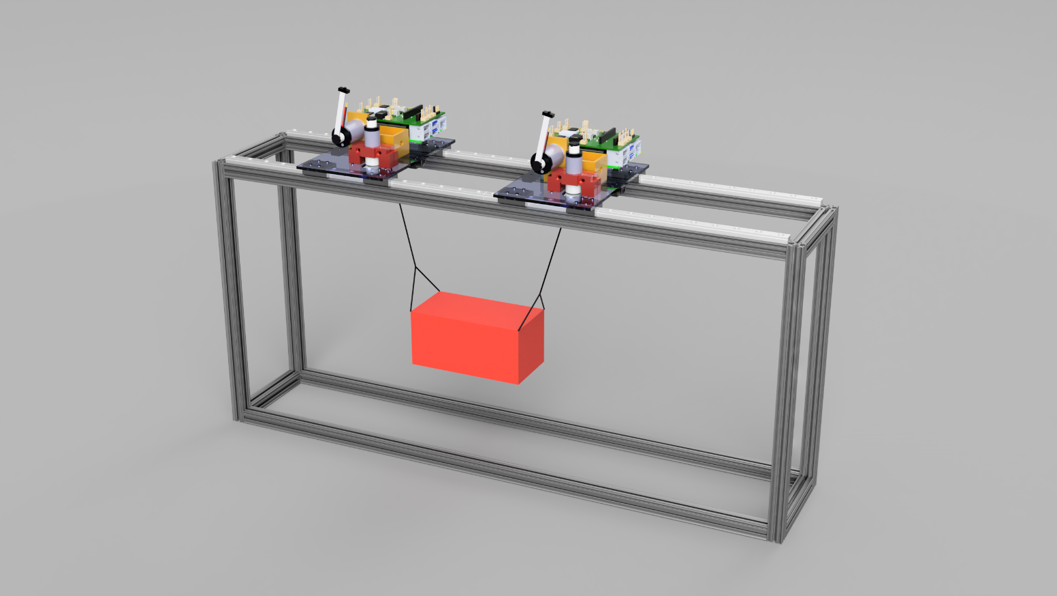
\includegraphics[width=110mm]{images/Veritas_demo_CAD}
	\end{center}

\end{frame}

%%%%%%%%%%%%%%%%%%%%%%%%%%%%%%%%%%%%%%%%%%%%%%%%%%%%%%%%%%%%

\begin{frame}<1>[label=sysbeschr2]
	\frametitle{System- {\color<1-3>{mygray} und Problembeschreibung}}
	\begin{center}
		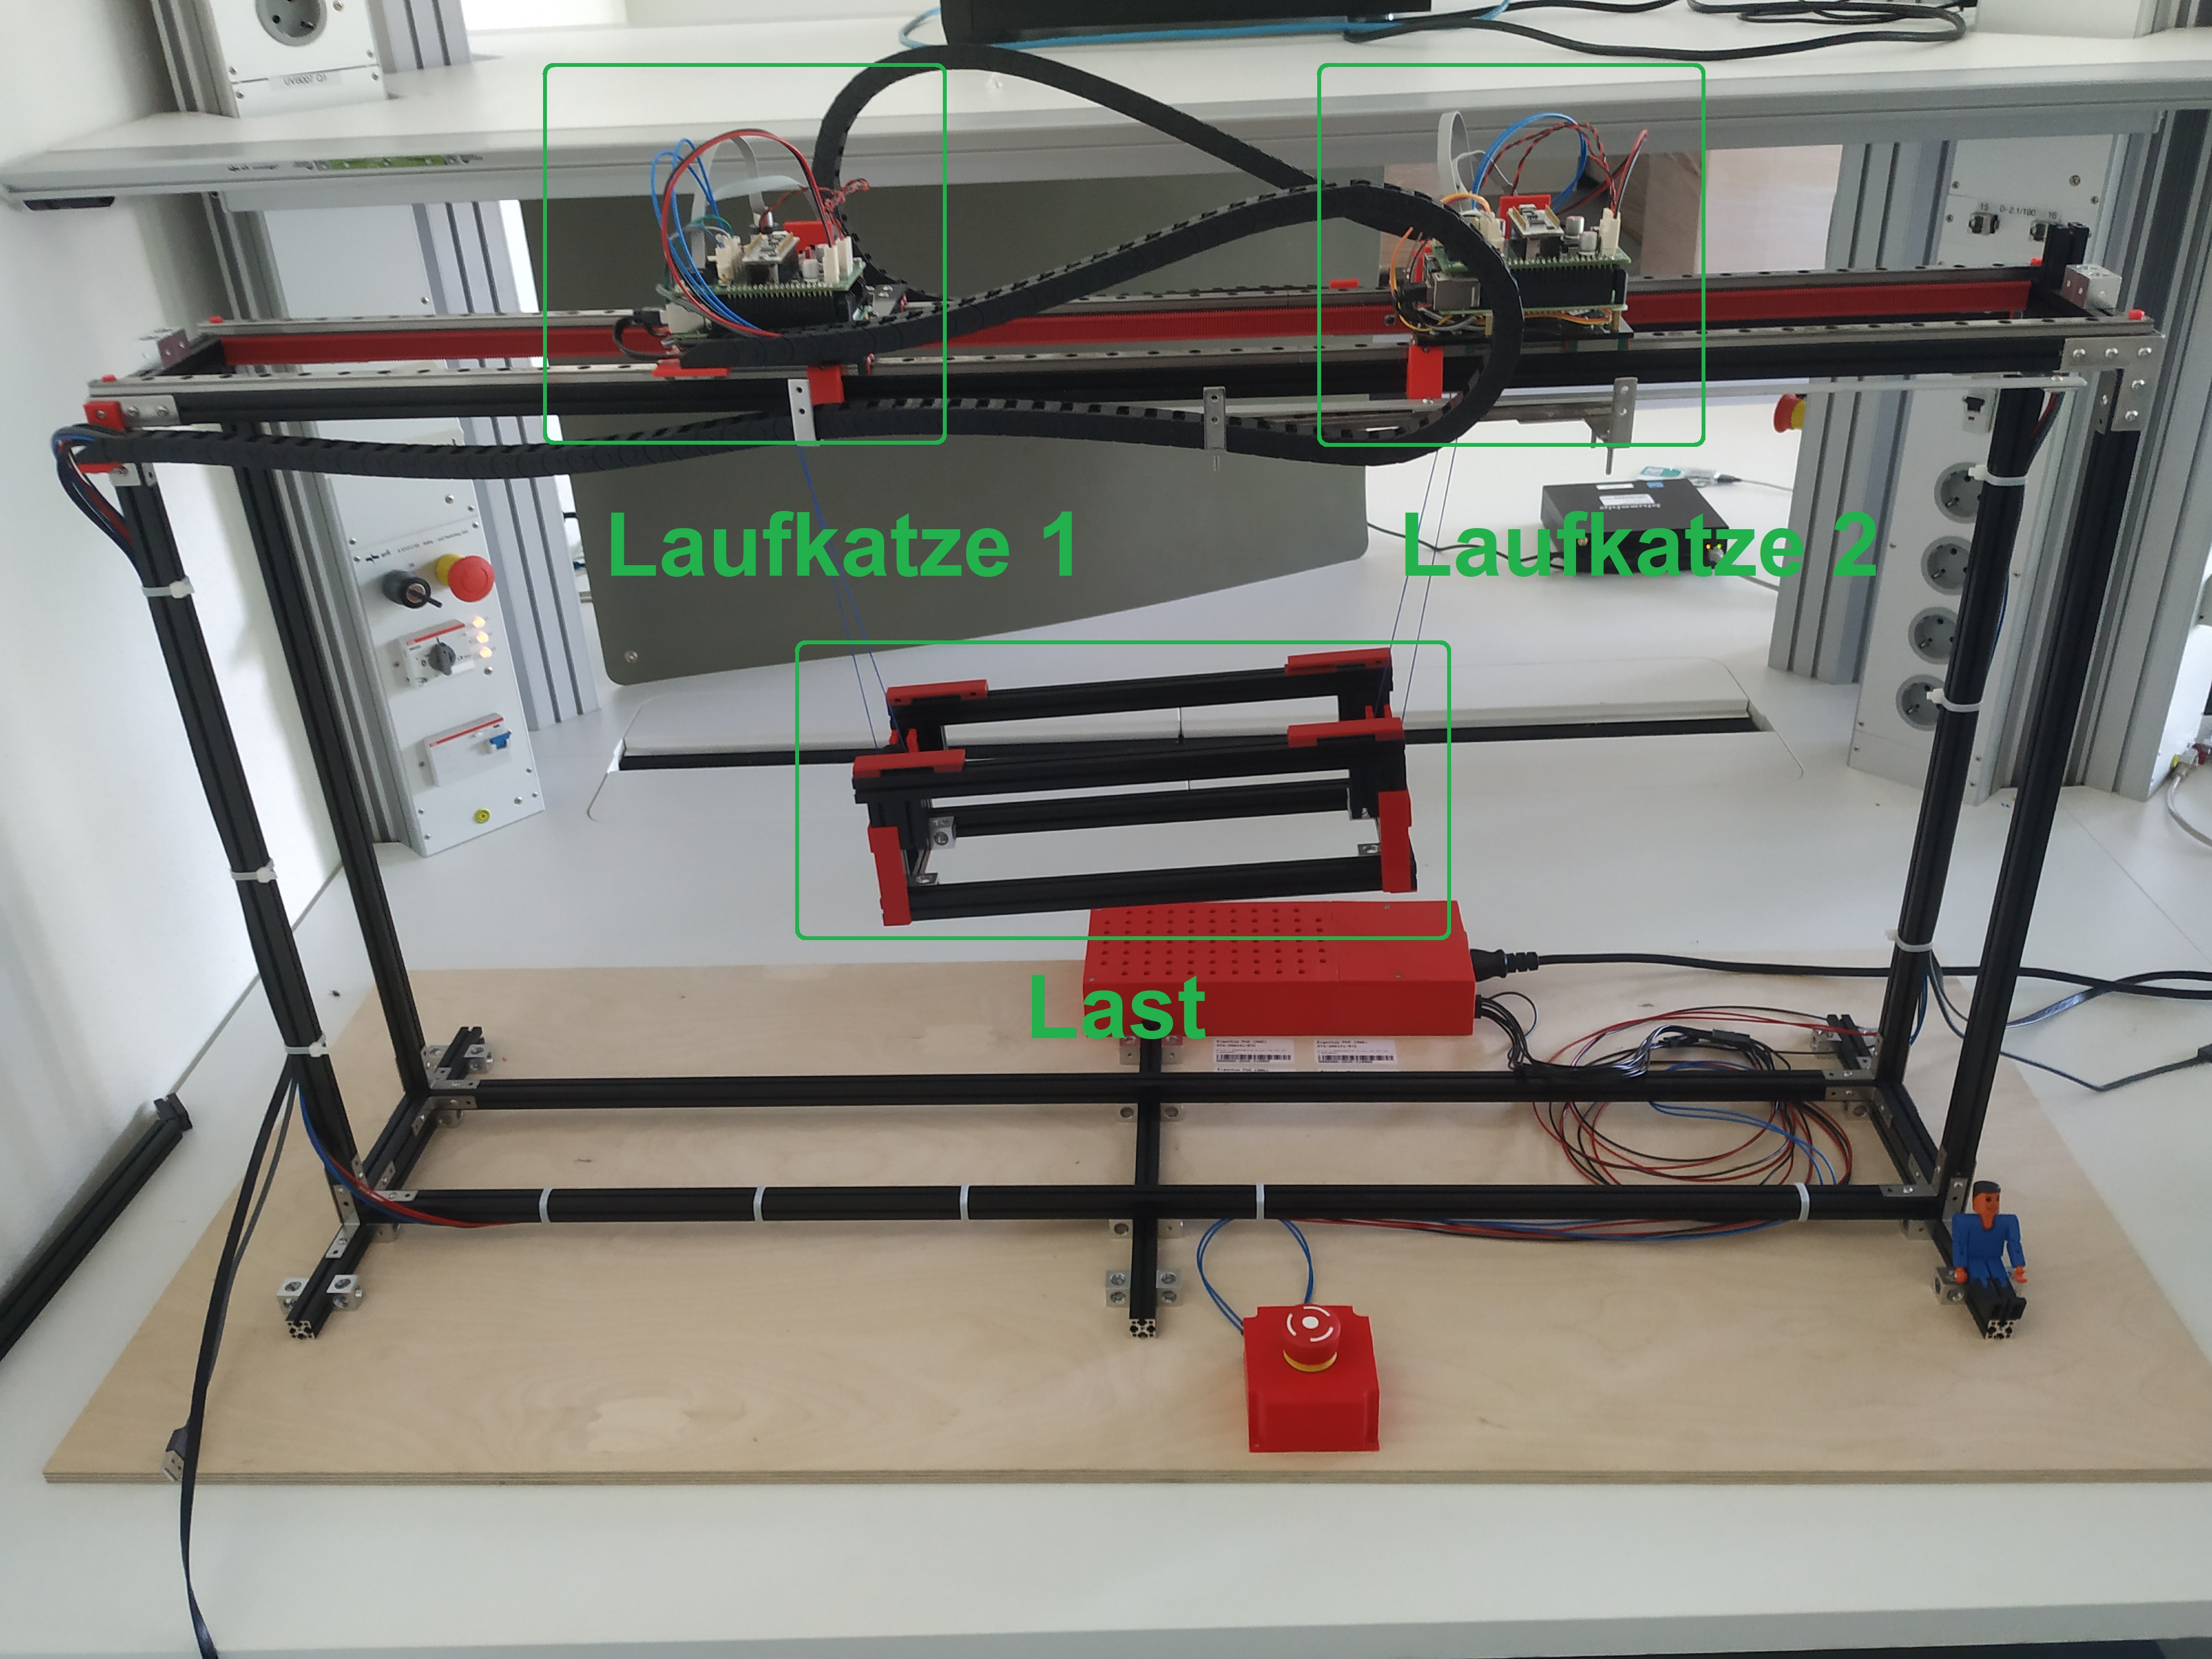
\includegraphics[width=85mm]{images/real_gantry}
	\end{center}
	
\end{frame}

%%%%%%%%%%%%%%%%%%%%%%%%%%%%%%%%%%%%%%%%%%%%%%%%%%%%%%%%%%%%

\begin{frame}[label=sysbeschr3]
	\frametitle{System- und Problembeschreibung}
	\textbf{Zielsetzung:}
	\begin{itemize}
		\item Ruckarme Überführung der Last zwischen Ruhelagen in der vertikalen Aufhängungsebene
		\pause
		\item Zentrale Trajektorienplanung und Referenzregelstrategie unter Vorgabe von Sollposen der Last
		\pause
		\item Regelungsentwurf auf Basis von Modellierung des Versuchsstands als Mehrkörpersystem
		\pause  
		\item Perspektivisch Vergleich der zentralen Regelung mit verteilten Regelungsansätzen und Grundlage für maschinelles Lernen 
	\end{itemize}
\end{frame}

%%%%%%%%%%%%%%%%%%%%%%%%%%%%%%%%%%%%%%%%%%%%%%%%%%%%%%%%%%%%

\begin{frame}<1>[label=gl2]
	\frametitle{Gliederung}
	\begin{itemize}
		%0
		\item[\cdbox] System- und Problembeschreibung
		%1
		\item[\only<1>{$\rightarrow$}\only<2>{$\rightarrow$}\only<3->{\cdbox}]
		\textbf<1>{Analytische Modellbildung}
		%2
		\item[\only<1>{$\square$}\only<2>{$\rightarrow$}\only<3->{\cdbox}]
		\textbf<2>{Flachheitsanalyse}
		%3
		\item[\only<1-2>{$\square$}\only<3>{$\rightarrow$}\only<4->{\cdbox}]
		\textbf<3>{Steuerungs- und Regelungsentwurf}
		%4
		\item[\only<1-2>{$\square$}\only<3>{$\rightarrow$}\only<4->{\cdbox}]
		\textbf<3>{Zusammenfassung und Ausblick}
	\end{itemize}
\end{frame}

%%%%%%%%%%%%%%%%%%%%%%%%%%%%%%%%%%%%%%%%%%%%%%%%%%%%%%%%%%%%

\begin{frame}[label=analMB]
	\frametitle{Analytische Modellbildung}
	\textbf{Allgemeine Modellannahmen:}
	\begin{itemize}
		\item Bewegung des Systems auf vertikale Ebene beschränkt
		\pause
		\item Seile mit vernachlässigbarer Masse gegenüber Laufkatzen, Last
		\pause
		\item Last trotz Aussparungen mit homogener Masseverteilung modelliert
		\pause
		\item Vernachlässigung dissipativer Kräfte 
	\end{itemize}

	\pause
	\bigskip
	\textbf{Vorgehen bei der Modellierung:}
	\begin{itemize}
		\item Modellierung Einzelkran mit Lagrange-Gleichungen zweiter Art (LG2)
		\pause
		\item Modellierung Doppelkran mit LG2
		\pause
		\item[$\rightarrow$] ODE-System: gut geeignet für Flachheitsnachweis, Simulation 
		\pause
		\item (Modellierung Doppelkran mit Lagrange-Gleichungen erster Art)
		\item[$\rightarrow$] (DAE-System: intuitive Zwangsbedingungen)
	\end{itemize}
\end{frame}

%%%%%%%%%%%%%%%%%%%%%%%%%%%%%%%%%%%%%%%%%%%%%%%%%%%%%%%%%%%%

\begin{frame}[t,fragile,label=ModellEinzelkran_2]{\large Analytisches Modell Einzelkran}
	\begin{textblock*}{80mm}[0.,0.](12mm,13mm)	
		\visible<1->{
			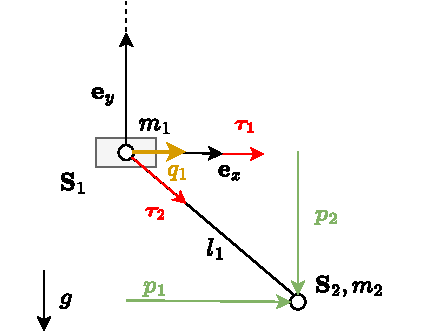
\includegraphics[width=64mm]{images/ODE_flatness_analysis_single_crane_diagram}
		}
		
		\visible<1->{
			\begin{itemize}
				\item Massen bei $\mathbf{S}_1 = (q_1, 0)^T$, $\mathbf{S}_2 = (p_1, p_2)^T$
				\item variable Seillänge $l_1 = \sqrt{(p_1 - q_1)^2 + p_2^2}$\\
				~
			\end{itemize}
		}
	\end{textblock*}
	
	\begin{textblock*}{80mm}[0.,0.](80mm,25mm)
		
		\visible<2->{
			\centering{\textbf{Systemgleichungen aus LG2:}}
			\begin{subequations}
				\label{single_flat_syseqs}
				\begin{flalign*}
					m_{2} \ddot{p}_{1} - \frac{\tau_{2} \left(p_{1} - q_{1}\right)}{l_{1}} &= 0\\
					g m_{2} + m_{2} \ddot{p}_{2} - \frac{p_{2} \tau_{2}}{l_{1}} &= 0\\
					m_{1} \ddot{q}_{1} - \tau_{1} + \frac{\tau_{2} \left(p_{1} - q_{1}\right)}{l_{1}} &= 0
				\end{flalign*}
			\end{subequations}
		}
		
	\end{textblock*}
	
\end{frame}

%%%%%%%%%%%%%%%%%%%%%%%%%%%%%%%%%%%%%%%%%%%%%%%%%%%%%%%%%%%%

\begin{frame}[t,fragile,label=ModellDoppelkran_2]{\large Analytisches Modell Doppelkran}
	\begin{textblock*}{80mm}[0.,0.](12mm,13mm)	
		\visible<1->{
			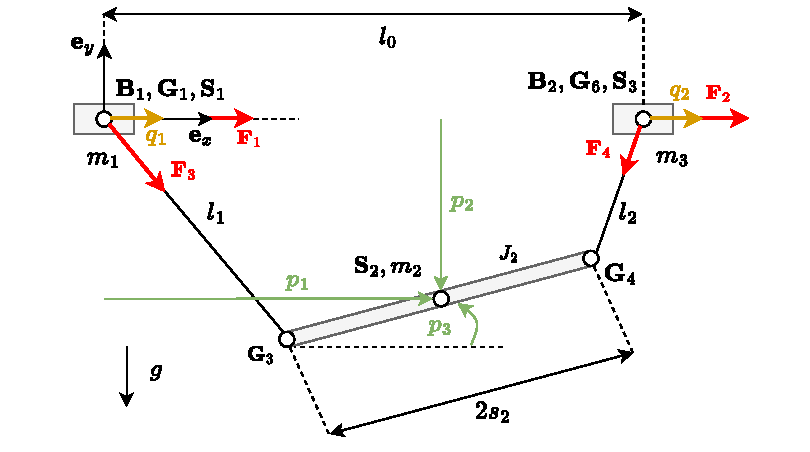
\includegraphics[width=64mm]{images/ODE_flatness_analysis_double_crane_diagram}
		}
		\bigskip
		\visible<1->{
			\textbf{variable Seillängen:}
			\tiny{
				\begin{flalign*}
					l_1 &= \sqrt{\left(p_{2} - s_{2} \sin{\left(p_{3} \right)}\right)^{2} + \left(p_{1} - q_{1} - s_{2} \cos{\left(p_{3} \right)}\right)^{2}}&& \\
					l_2 &= \sqrt{\left(p_{2} + s_{2} \sin{\left(p_{3} \right)}\right)^{2} + \left(- l_{0} + p_{1} - q_{2} + s_{2} \cos{\left(p_{3} \right)}\right)^{2}}&&
				\end{flalign*}
			}
			~
		}
	\end{textblock*}

	\begin{textblock*}{80mm}[0.,0.](80mm,20mm)	
		\visible<2->{
			\textbf{Systemgleichungen aus LG2:}
			\tiny{
			\begin{flalign*}
			&m_{2} \ddot{p}_{1} - \frac{\tau_{4} \left(- l_{0} + p_{1} - q_{2} + s_{2} \cos{p_{3}}\right)}{l_{2}} - \frac{\tau_{3} \left(p_{1} - q_{1} - s_{2} \cos{p_{3}}\right)}{l_{1}} = 0\\
			&g m_{2} + m_{2} \ddot{p}_{2} - \frac{\tau_{4} \left(p_{2} + s_{2} \sin{p_{3}}\right)}{l_{2}} - \frac{\tau_{3} \left(p_{2} s_{2} \sin{p_{3}}\right)}{l_{1}} = 0\\
			&J_{2} \ddot{p}_{3} - \frac{s_{2} \tau_{4} \left(p_{2} + s_{2} \sin{p_{3}}\right) \cos{p_{3}} + s_{2} \tau_{4} \left(p_{1} - q_{2} + s_{2} \cos{p_{3}} - l_{0} \right)}{l_{2}}\\
			&+ \frac{s_{2} \tau_{3} \left(p_{2} - s_{2} \sin{p_{3}}\right) \cos{p_{3}}}{l_{1}} - \frac{s_{2} \tau_{3} \left(p_{1} - q_{1} - s_{2} \cos{p_{3}}\right) \sin{p_{3}}}{l_{1}} = 0\\
			&m_{1} \ddot{q}_{1} - \tau_{1} + \frac{\tau_{3} \left(p_{1} - q_{1} - s_{2} \cos{p_{3}}\right)}{l_{1}} = 0\\
			&m_{3} \ddot{q}_{2} - \tau_{2} + \frac{\tau_{4} \left(- l_{0} + p_{1} - q_{2} + s_{2} \cos{p_{3}}\right)}{l_{2}} = 0
			\end{flalign*}
			}
		}
		
	\end{textblock*}
	
\end{frame}

%%%%%%%%%%%%%%%%%%%%%%%%%%%%%%%%%%%%%%%%%%%%%%%%%%%%%%%%%%%%
\begin{frame}[t,fragile,label=ModellDoppelkran_3]{\large Analytisches Modell Doppelkran}
	\begin{textblock*}{80mm}[0.,0.](12mm,13mm)	
		\visible<1->{
			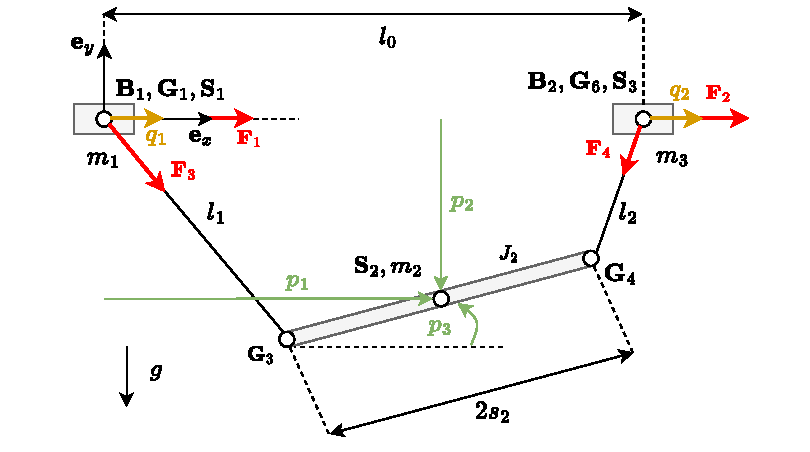
\includegraphics[width=64mm]{images/ODE_flatness_analysis_double_crane_diagram}
		}
		\bigskip
		\visible<1->{
			\textbf{variable Seillängen:}
			\tiny{
				\begin{flalign*}
					l_1 &= \sqrt{\left(p_{2} - s_{2} \sin{\left(p_{3} \right)}\right)^{2} + \left(p_{1} - q_{1} - s_{2} \cos{\left(p_{3} \right)}\right)^{2}}&& \\
					l_2 &= \sqrt{\left(p_{2} + s_{2} \sin{\left(p_{3} \right)}\right)^{2} + \left(- l_{0} + p_{1} - q_{2} + s_{2} \cos{\left(p_{3} \right)}\right)^{2}}&&
				\end{flalign*}
			}
			~
		}
	\end{textblock*}
	
	\begin{textblock*}{80mm}[0.,0.](80mm,13mm)
		
		\visible<1->{	
			\textbf{Eingangsaffines Zustandsraummodell:}			
		\begin{align*}
			\begin{split}
				\dot{\mathbf{x}} &= \mathbf{f}(\mathbf{x}) + \mathbf{g}(\mathbf{x}) \boldsymbol{\tau} \text{ mit } \\ 
				\mathbf{x} &= (p_{1},	p_{2}, p_{3}, q_{1}, q_{2}, \dot{p}_{1}, \dot{p}_{2}, \dot{p}_{3}, \dot{q}_{1}, \dot{q}_{2})^T, \\
				\mathbf{f}(\mathbf{x}) &= 
				(\dot{p}_{1}, \dot{p}_{2}, \dot{p}_{3}, \dot{q}_{1}, \dot{q}_{2}, 0, -g, 0, 0, 0)^T, \\ 
				\mathbf{g}(\mathbf{x}) &=
				\left(\begin{matrix}
					0 & 0 & 0 & 0\\
					0 & 0 & 0 & 0\\
					0 & 0 & 0 & 0\\
					0 & 0 & 0 & 0\\
					0 & 0 & 0 & 0\\
					0 & 0 & * & *\\
					0 & 0 & * & *\\
					0 & 0 & * & *\\
					* & 0 & * & 0\\
					0 & * & 0 & *
				\end{matrix}\right) \ \text{wobei} \ * \neq 0 
			\end{split}
		\end{align*}
		}
	\end{textblock*}
	
\end{frame}

%%%%%%%%%%%%%%%%%%%%%%%%%%%%%%%%%%%%%%%%%%%%%%%%%%%%%%%%%%%%

\begin{frame}<1>[label=gl3]
	\frametitle{Gliederung}
	\begin{itemize}
		%0
		\item[\cdbox] System- und Problembeschreibung
		%1
		\item[\cdbox] Analytische Modellbildung
		%2
		\item[\only<1>{$\rightarrow$}\only<2>{$\rightarrow$}\only<3->{\cdbox}]
		\textbf<1>{Flachheitsanalyse}
		%3
		\item[\only<1-2>{$\square$}\only<3>{$\rightarrow$}\only<4->{\cdbox}]
		\textbf<2>{Steuerungs- und Regelungsentwurf}
		%4
		\item[\only<1-2>{$\square$}\only<3>{$\rightarrow$}\only<4->{\cdbox}]
		\textbf<3>{Zusammenfassung und Ausblick}
	\end{itemize}
\end{frame}

%%%%%%%%%%%%%%%%%%%%%%%%%%%%%%%%%%%%%%%%%%%%%%%%%%%%%%%%%%%%

\begin{frame}[label=Flachheit_1]
	\frametitle{Flachheitsanalyse}
   	\begin{block}{Differenzielle Flachheit}
	Ein System der Form $\dot{\mathbf{x}} = \mathbf{F}(\mathbf{x}, \mathbf{u})$ mit $\mathbf{F}, \mathbf{x} \in \mathbb{R}^n$ und $\mathbf{u} \in \mathbb{R}^m$ heißt (differenziell) flach, falls ein $m$-Tupel $y := (y_1, ..., y_m)^T$ sowie glatte Funktionen $\mathbf{\Psi}$, $\boldsymbol{\theta}$ existieren, so dass
	\begin{align*}
			\mathbf{x} &= \mathbf{\Psi}(\mathbf{y}, \dot{\mathbf{y}}, ..., \mathbf{y}^{(n_x)}) \text{ mit } n_x < \infty \text{ und } \\
			\mathbf{u} &= \boldsymbol{\theta}(\mathbf{y}, \dot{\mathbf{y}}, ..., \mathbf{y}^{(n_u)}) \text{ mit } n_u < \infty \text{ gilt.}
	\end{align*}
	\end{block}

	\pause
	\bigskip
	\textbf{Erläuterungen:}
	\begin{itemize}
		\item Systemzustand $\mathbf{x}$, Systemeingang $\mathbf{u}$ 
		\item \textbf{flacher Ausgang} $\mathbf{y}$
		\item[$\rightarrow$] Parametrisierung aller Systemgrößen durch $\mathbf{y}$ und endlich viele Ableitungen ohne Lösung von DGL/Integration möglich
	\end{itemize}
\end{frame}

%%%%%%%%%%%%%%%%%%%%%%%%%%%%%%%%%%%%%%%%%%%%%%%%%%%%%%%%%%%%

\begin{frame}[t,fragile,label=Flachheit_2]{\large Flachheitsanalyse von MIMO-Systemen}
	
	\textbf{Prinzipielles Vorgehen:}
	\begin{itemize}
		\pause
		\item  nichtlineares MIMO-System mit Zustand $\mathbf{x} \in \mathbb{R}^n$ und Eingang $\mathbf{u} \in \mathbb{R}^m$
		\pause
		\item sukzessive Elimination der $m$ Komponenten von $\mathbf{u}$ durch je eine der $n$ Systemgleichungen
		\pause
		\item[$\rightarrow$] anschließend analog Elimination von $n - m$ Komponenten von $\mathbf{x}$
		\pause
		\item[$\rightarrow$] übrig bleiben $n - (n - m) = m $ Zustandskomponenten als \textbf{flacher Ausgang} $\mathbf{y}$
	\end{itemize}
	
	\bigskip
	\pause
	
	\textbf{Parametrisierung der Systemgrößen durch den flachen Ausgang:}
	\begin{itemize}
		\pause
		\item Systemgleichungen in Umgekehrter Reihenfolge zur Elimination nach Systemgrößen auflösen
		\pause
		\item Parametrisierungen vorheriger Größen oder deren Zeitableitungen ggf. in folgende Parametrisierungen einsetzen
	\end{itemize}
\end{frame}

%%%%%%%%%%%%%%%%%%%%%%%%%%%%%%%%%%%%%%%%%%%%%%%%%%%%%%%%%%%%

\begin{frame}[t,fragile,label=Flachheit_Einzelkran_new1]{\large Flachheitsanalyse am Einzelkran}
	
	\begin{textblock*}{80mm}[0.,0.](115mm,5mm)	
	\visible<1->{
		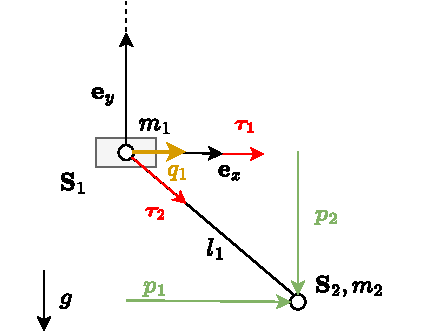
\includegraphics[width=44mm]{images/ODE_flatness_analysis_single_crane_diagram}
	}
	\end{textblock*}
	
	\textbf{Elimination von Systemgrößen- und Gleichungen:}
	
	\begin{itemize}
		\item Elimination der Eingangskomponenten von $\mathbf{u} = (\tau_1, \tau_2)^T$:
		\begin{align*}
		\begin{split}
			m_{2} \ddot{p}_{1} - \frac{\textcolor{blue}{\tau_{2}} \left(p_{1} - q_{1}\right)}{l_{1}} &= 0\\
			g m_{2} + m_{2} \ddot{p}_{2} - \frac{p_{2} \tau_{2}}{l_{1}} &= 0\\
			m_{1} \ddot{q}_{1} - \textcolor{red}{\tau_{1}} + \frac{\tau_{2} \left(p_{1} - q_{1}\right)}{l_{1}} &= 0
		\end{split}
		\end{align*}
		\pause
		\item[$\rightarrow$] Elimination von $\textcolor{red}{\tau_{1}}$ und 3. Gleichung
		\pause
		\item[$\rightarrow$] Elimination von $\textcolor{blue}{\tau_{2}}$ und 1. Gleichung
		\pause
		\item[$\rightarrow$] Einsetzen von $\textcolor{blue}{\tau_{2}}$ aus 1. Gleichung in 2. Gleichung:
		\begin{align*}
			g m_{2} + m_{2} \ddot{p}_{2} - \frac{m_2 p_{2} \ddot{p}_1}{p_1 - q_1} = 0
		\end{align*}
	\end{itemize}
	
\end{frame}

%%%%%%%%%%%%%%%%%%%%%%%%%%%%%%%%%%%%%%%%%%%%%%%%%%%%%%%%%%%%

\begin{frame}[t,fragile,label=Flachheit_Einzelkran_new2]{\large Flachheitsanalyse am Einzelkran}
	
	\begin{textblock*}{80mm}[0.,0.](115mm,5mm)	
		\visible<1->{
			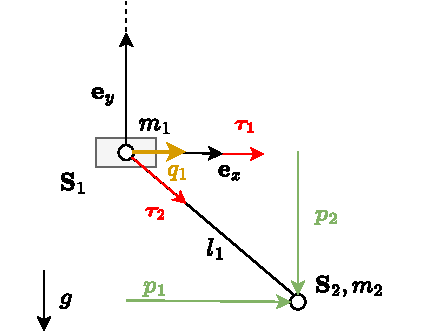
\includegraphics[width=44mm]{images/ODE_flatness_analysis_single_crane_diagram}
		}
	\end{textblock*}
	
	\textbf{Elimination von Systemgrößen- und Gleichungen:}
	
	\begin{itemize}
		\item[$\rightarrow$] Einsetzen von $\textcolor{blue}{\tau_{2}}$ aus 1. Gleichung in 2. Gleichung:
		\begin{align*}
		g m_{2} + m_{2} \ddot{p}_{2} - \frac{m_2 p_{2} \ddot{p}_1}{p_1 - \textcolor{green}{q_1}} = 0
		\end{align*}
		\item[$\rightarrow$] folgende Menge an Systemgrößen $\mathcal{M} = \{p_1, \ddot{p}_1, p_2, \ddot{p}_2, q_1 \}$
		\pause
		\item[$\rightarrow$] Elimination von $q_1$, da rein algebraisch $\rightarrow$ $\mathbf{y} = (p_1, p_2)^T$
	\end{itemize}
	
	\bigskip
	\pause
	
	\textbf{Parametisierung der Systemgrößen durch $\mathbf{y} = (p_1, p_2)^T$:}
	\begin{itemize}
		\item aus 2. substituierter Gleichung: $\textcolor{green}{q_1} = \frac{g p_{1} + p_{1} \ddot{p}_{2} - p_{2} \ddot{p}_{1}}{g + \ddot{p}_{2}}$
		\pause 
		\item aus 1. Gleichung und Einsetzen von $\textcolor{green}{q_1}(\mathbf{y}, \ddot{\mathbf{y}})$: 
		\begin{equation*}
			m_{2} \ddot{p}_{1} - \frac{\textcolor{blue}{\tau_{2}} \left(p_{1} - \textcolor{green}{q_1}\right)}{l_{1}} = 0
			\quad \Rightarrow \quad
			\textcolor{blue}{\tau_{2}} = \frac{m_{2} \ddot{p}_{1} \sqrt{p_{2}^{2} + \left(p_{1} - \frac{g p_{1} + p_{1} \ddot{p}_{2} - p_{2} \ddot{p}_{1}}{g + \ddot{p}_{2}}\right)^{2}}}{p_{1} - \frac{g p_{1} + p_{1} \ddot{p}_{2} - p_{2} \ddot{p}_{1}}{g + \ddot{p}_{2}}}
		\end{equation*}
	\end{itemize}
	
	
\end{frame}

%%%%%%%%%%%%%%%%%%%%%%%%%%%%%%%%%%%%%%%%%%%%%%%%%%%%%%%%%%%%

\begin{frame}[t,fragile,label=Flachheit_Einzelkran_new3]{\large Flachheitsanalyse am Einzelkran}
	
	\begin{textblock*}{80mm}[0.,0.](115mm,5mm)	
		\visible<1->{
			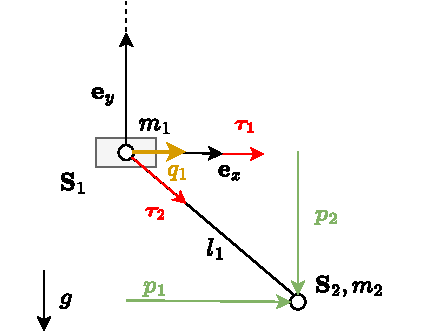
\includegraphics[width=44mm]{images/ODE_flatness_analysis_single_crane_diagram}
		}
	\end{textblock*}
	
	\textbf{Parametisierung der Systemgrößen durch $\mathbf{y} = (p_1, p_2)^T$:}
	\begin{itemize}
		\item aus 3. Gleichung und Einsetzen von $\textcolor{green}{q_1}$, $\textcolor{green}{\ddot{q}_1}$, $\textcolor{blue}{\tau_2}$:  
		\begin{align*}
		0 &= m_{1} \textcolor{green}{\ddot{q}_1} - \textcolor{red}{\tau_{1}} + \frac{\textcolor{blue}{\tau_2} \left(p_{1} - \textcolor{green}{\ddot{q}_1}\right)}{l_{1}} \\
		\Rightarrow
		\textcolor{red}{\tau_1} &=
		\frac{1}{g^{3} + 3 g^{2} \ddot{p}_{2} + 3 g \ddot{p}_{2}^{2} + \ddot{p}_{2}^{3}}
		(g^{3} m_{1} \ddot{p}_{1} + g^{3} m_{2} \ddot{p}_{1} - g^{2} m_{1} p_{2} \ddddot{p}_{1}\\ 
		&- 2 g^{2} m_{1} \dddot{p}_{1} \dot{p}_{2} + 2 g^{2} m_{1} \ddot{p}_{1} \ddot{p}_{2} + 3 g^{2} m_{2} \ddot{p}_{1} \ddot{p}_{2} - 2 g m_{1} p_{2} \ddddot{p}_{1} \ddot{p}_{2} + g m_{1} p_{2} \ddddot{p}_{2} \ddot{p}_{1} \\ 
		&+ 2 g m_{1} p_{2} \dddot{p}_{1} \dddot{p}_{2} - 4 g m_{1} \dddot{p}_{1} \ddot{p}_{2} \dot{p}_{2} + 2 g m_{1} \dddot{p}_{2} \ddot{p}_{1} \dot{p}_{2} + g m_{1} \ddot{p}_{1} \ddot{p}_{2}^{2} + 3 g m_{2} \ddot{p}_{1} \ddot{p}_{2}^{2} - m_{1} p_{2} \ddddot{p}_{1} \ddot{p}_{2}^{2}\\ 
		&+ m_{1} p_{2} \ddddot{p}_{2} \ddot{p}_{1} \ddot{p}_{2} + 2 m_{1} p_{2} \dddot{p}_{1} \dddot{p}_{2} \ddot{p}_{2} - 2 m_{1} p_{2} \dddot{p}_{2}^{2} \ddot{p}_{1} - 2 m_{1} \dddot{p}_{1} \ddot{p}_{2}^{2} \dot{p}_{2} + 2 m_{1} \dddot{p}_{2} \ddot{p}_{1} \ddot{p}_{2} \dot{p}_{2} + m_{2} \ddot{p}_{1} \ddot{p}_{2}^{3})
		\end{align*}
		\bigskip
		\pause
		\item[$\rightarrow$] alle Systemgrößen durch flachen Ausgang $\mathbf{y} = (p_1, p_2)^T$ parametrisiert
		\pause
		\item[$\rightarrow$] konstruktiver Flachheitsnachweis erbracht \quad $\Box$
	\end{itemize}
	
	
\end{frame}

%%%%%%%%%%%%%%%%%%%%%%%%%%%%%%%%%%%%%%%%%%%%%%%%%%%%%%%%%%%%

\begin{frame}[t,fragile,label=Flachheit_Doppelkran_1]{\large Flachheitsanalyse am Doppelkran}
	
	\textbf{Elimination von Systemgrößen- und Gleichungen:}
	
	\begin{itemize}
		\item Vorgehen analog zum Einzelkran
		\pause
		\item[$\rightarrow$] unpraktikable Darstellung umfangreicher Terme, über CAS \textit{SymPy} durchgeführt
		\pause
		\bigskip
		\item $n = 10$ Zustandskomponenten und -gleichungen, $m = 4$ Eingangskomponenten
		\pause
		\item[$\rightarrow$] Elimination des Eingangs, autonomes System aus $p = n - m = 6$ Gleichungen
		\pause
		\item[$\rightarrow$] Elimination von $p$ Zuständen zu flachem Ausgang aus $m = 4$ Komponenten
		\pause
		\bigskip
		\item letzte übrige Gleichung enthält folgende Menge an Systemgrößen:
		\begin{equation*}
			\mathcal{M} = \{p_1, p_2, p_3, \ddot{p}_1, \ddot{p}_2, \ddot{p}_3, q_1, q_2 \}
		\end{equation*}
		\pause
		\item[$\rightarrow$] algebraisches Auftreten von $q_1$, $q_2$ führt o. B. d. A. zur Wahl von $\mathbf{y} = (p_1, p_2, p_3, q_1)^T$
	\end{itemize}
	
\end{frame}

%%%%%%%%%%%%%%%%%%%%%%%%%%%%%%%%%%%%%%%%%%%%%%%%%%%%%%%%%%%%

\begin{frame}[t,fragile,label=Flachheit_Doppelkran_2]{\large Flachheitsanalyse am Doppelkran}
	
	\textbf{Parametisierung der Systemgrößen durch $\mathbf{y} = (p_1, p_2, p_3, q_1)^T:$}
		
	\begin{itemize}
		\item funktionale Zusammenhänge der Parametrisierungen:
		\begin{align*}
			\tau_1 &= \theta_1 \left(p_1, \ddot{p}_1, p_2, \ddot{p}_2, p_3, \ddot{p}_3, q_1, \ddot{q}_1 \right) \\
			\tau_2 &= \theta_2 \left(p_1, \dot{p}_1, \ddot{p}_1, p_1^{(3)}, p_1^{(4)}, p_2, \dot{p}_2, \ddot{p}_2, p_2^{(3)}, p_2^{(4)}, p_3, \dot{p}_3, \ddot{p}_3, p_3^{(3)}, p_3^{(4)}, q_1, \dot{q}_1, \ddot{q}_1 \right) \\
			\tau_3 &= \theta_3 \left(p_1, \ddot{p}_1, p_2, \ddot{p}_2, p_3, \ddot{p}_3, q_1 \right) \\
			\tau_4 &= \theta_4 \left(p_1, \ddot{p}_1, p_2, \ddot{p}_2, p_3, \ddot{p}_3, q_1 \right) \\
			q_2 &= \Psi_1 \left(p_1, \ddot{p}_1, p_2, \ddot{p}_2, p_3, \ddot{p}_3, q_1 \right)
		\end{align*}
		\pause
		\item[$\rightarrow$] alle Systemgrößen durch flachen Ausgang $\mathbf{y} = (p_1, p_2, p_3, q_1)^T$ parametrisiert \quad $\Box$
	\end{itemize}
		
\end{frame}

%%%%%%%%%%%%%%%%%%%%%%%%%%%%%%%%%%%%%%%%%%%%%%%%%%%%%%%%%%%%

\begin{frame}<1>[label=gl4]
	\frametitle{Gliederung}
	\begin{itemize}
		%0
		\item[\cdbox] System- und Problembeschreibung
		%1
		\item[\cdbox] Analytische Modellbildung
		%2
		\item[\cdbox] Flachheitsanalyse
		%3
		\item[\only<1>{$\rightarrow$}\only<2>{$\rightarrow$}\only<4->{\cdbox}]
		\textbf<1>{Steuerungs- und Regelungsentwurf}
		%4
		\item[\only<1-2>{$\square$}\only<3>{$\rightarrow$}\only<4->{\cdbox}]
		\textbf<3>{Zusammenfassung und Ausblick}
	\end{itemize}
\end{frame}

%%%%%%%%%%%%%%%%%%%%%%%%%%%%%%%%%%%%%%%%%%%%%%%%%%%%%%%%%%%%

\begin{frame}[label=control]
	\frametitle{Steuerungs- und Regelungsentwurf}
	\textbf{Allgemeines Vorgehen:}
	\begin{itemize}
		\item Planung polynombasierter Referenztrajektorien für den flachen Ausgang $\mathbf{y}$
		\pause
		\item Trajektorien der Systemeingänge $\boldsymbol{\tau}(t)$ folgen aus $\mathbf{y}(t)$
		\pause
		\item[$\rightarrow$] Vor\textbf{steuerung} durch Parametrisierung aus Flachheitsnachweis möglich
		\pause
		\item Entwurf einer Folge\textbf{regelung} um diese Trajektorien
	\end{itemize}

\end{frame}

%%%%%%%%%%%%%%%%%%%%%%%%%%%%%%%%%%%%%%%%%%%%%%%%%%%%%%%%%%%%

\begin{frame}[t,fragile,label=trajektorien_1]{\large Trajektorienplanung}
	
	\textbf{Anforderungen:}
	\begin{itemize}
		\pause
		\item Überführung des Doppelkransystems zwischen zwei Ruhelagen
		\pause
		\item stetiger Verlauf von Eingangs- bzw. Stellgrößen
		\pause
		\item bisher keine formal spezifizierten Grenzwerte für Beschleunigungen etc.
	\end{itemize}
	
	\pause
	\bigskip
	\textbf{Vorgabe von Randbedingungen:}
	\begin{itemize}
		\pause
		\item Differenzierbarkeitsbedingungen an $\mathbf{y}(t)$ folgen aus $\boldsymbol{\tau}(\mathbf{y}(t), \dot{\mathbf{y}}(t), ...)$
		\pause
		\item[$\rightarrow$] höchste Ableitungen von $\mathbf{y}(t)$ in $\tau_2 = \theta_2 \left(y_1^{(4)}, y_2^{(4)}, y_3^{(4)}, \ddot{y}_4, ... \right)$
		\pause
		\item[$\rightarrow$] stetig differenzierbarer Verlauf von $\boldsymbol{\tau}(t)$ für Überführung von $(t_0, y_{i, 0})$ in $(t_e, y_{i, e})$
		\pause
		\item[$\rightarrow$] 2 x 3 bzw. 2 x 5 Randbedingungen für $y_i$ $\rightarrow$ Polynome der Ordnung 5 bzw. 9:
		\begin{align*}
			\begin{split}
				y_i(t) &= a_{i, 9} t^9 + a_{i, 8} t^8 + ... + a_{i, 0} \quad \text{für }  i = 1,2,3; \ t_0 < t < t_e \\
				y_4(t) &= a_{4, 5} t^5 + a_{4, 4} t^4 + ... + a_{4, 0} \quad \text{für } t_0 < t < t_e.
			\end{split}
		\end{align*}
		
	\end{itemize}
	
\end{frame}

%%%%%%%%%%%%%%%%%%%%%%%%%%%%%%%%%%%%%%%%%%%%%%%%%%%%%%%%%%%%

\begin{frame}[t,fragile,label=trajektorien_3]{\large Prototypische Referenztrajektorie}
	
	\begin{center}
    	\includemovie[attach=false,autoplay,text={%
    		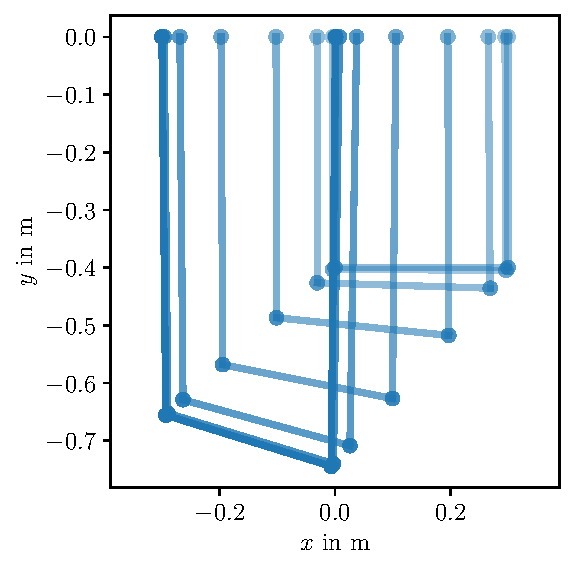
\includegraphics[width=0.6\textwidth]{images/onion_skinned_picture}%
    	}]{1.0\linewidth}{0.45\linewidth}{images/gantry_crane_trajectory.mp4}
    \end{center}
	
\end{frame}

%%%%%%%%%%%%%%%%%%%%%%%%%%%%%%%%%%%%%%%%%%%%%%%%%%%%%%%%%%%%

\begin{frame}[t,fragile,label=trajektorienregelung_2]{\large Trajektorienfolgeregelung}

	\begin{textblock*}{42mm}[0.,0.](115mm, 16mm)
		\visible<2->{
			\begin{tcolorbox}[colback=lightgray,colframe=softblue,title=Lie-Ableitung]
				$\dot{\mathbf{x}} = \mathbf{f}(\mathbf{x}) + \mathbf{g}(\mathbf{x}) \mathbf{u}$\\
				$\mathbf{y} = \mathbf{h}(\mathbf{x})$\\
				$ \Rightarrow L_{\mathbf{f}} h_i = \mathrm{d} h_i^T \cdot \mathbf{f}$
			\end{tcolorbox}
		}
	\end{textblock*}

	\begin{itemize}
		\item Bestimmung der Komponenten $r_i$ des \textbf{vektoriellen relativen Grades} $\mathbf{r}$:
	\end{itemize}
	\pause
	\begin{align*}
	y_i &= h_i(\mathbf{x}) \\
	\dot{y}_i &= L_{\mathbf{f}} h_i(\mathbf{x}) \\
	&\vdots \\
	y_i^{(r_i - 1)} &= L_{\mathbf{f}}^{r_i - 1} h_i(\mathbf{x}) \\
	y_i^{(r_i)} &= L_{\mathbf{f}}^{r_i} h_i(\mathbf{x}) + L_{\mathbf{g}_1} L_{\mathbf{f}}^{r_i - 1} h_i(\mathbf{x}) u_1 + \hdots + L_{\mathbf{g}_m} L_{\mathbf{f}}^{r_i - 1} h_i(\mathbf{x}) u_m
	\end{align*}
	\pause

	\begin{table}[htbp]%
		\centering
		%\caption{Relative Grade der Ausgänge und explizites Auftreten der Eingänge.}
		\label{tab:relative_degrees}
		\begin{tabular}{c| c c c c}
			\hline
			Index $i$ & 1 & 2 & 3 & 4 \\ 
			\hline
			Komponente des vektoriellen relativen Grades $r_i$ & 2 & 2 & 2 & 2\\ 
			\hline
			explizities Auftreten von $\tau_j$ bei $y_i^{(r_i)}$ & $\tau_3, \tau_4$ & $\tau_3, \tau_4$ & $\tau_3, \tau_4$ & $\tau_1, \tau_3$ \\
			\hline
			$y_j^{(k)}$ mit minimalem $k$, bei dem $\tau_i$ zuerst auftritt & $y_4^{(2)}$ & \textcolor{red}{$y_{1,2,3}^{(4)}$} & $y_{1,2,3,4}^{(2)}$ & $y_{1,2,3}^{(2)}$\\
			\hline
		\end{tabular}
	\end{table}
	
\end{frame}

%%%%%%%%%%%%%%%%%%%%%%%%%%%%%%%%%%%%%%%%%%%%%%%%%%%%%%%%%%%%

\begin{frame}[t,fragile,label=trajektorienregelung_3]{\large Trajektorienfolgeregelung - Statische Rückführung}
	
	\begin{itemize}
		\item System mit Eingangs-Ausgangs-Verhalten der Form
	\end{itemize}
	\begin{equation*}
		\mathbf{y}^{(\mathbf{r})} = \boldsymbol{\Gamma}(\mathbf{x}) + \boldsymbol{\Lambda}(\mathbf{x}) \mathbf{u} \ \text{, } \ \boldsymbol{\Gamma}(\mathbf{x}) = (L_{\mathbf{f}}^{r_1} h_1(\mathbf{x}), ..., L_{\mathbf{f}}^{r_m} h_m(\mathbf{x}))^T
	\end{equation*}
	\pause
	\begin{itemize}
		\item Virtueller Eingang $\mathbf{v} \stackrel{!}{=} \mathbf{y}^{(\mathbf{r})}$ und Auflösen nach $\mathbf{u}$ (falls $\mathbf{r}$ wohldefiniert!)
	\end{itemize}
	\pause
	\begin{equation*}
		\Rightarrow \mathbf{u} = \boldsymbol{\Lambda }^{-1}(\mathbf{x}) \cdot (\mathbf{v} - \boldsymbol{\Gamma}(\mathbf{x})) \quad \textbf{(statische Rückführung)}
	\end{equation*}
	\begin{itemize}
		\item Wahl von $\mathbf{v}$ nach stabilisierender Fehlerdynamik von $e_i := y_i - y_{i, \text{ref}}$
	\end{itemize}
	\begin{align*}
			e_i^{(r_i)} + c_{i, r_i-1} \ e_i^{(r_i-1)} + ... + c_{i, 1} \ \dot{e}_i + c_{i, 0} \ e_i = 0 \\
			\Leftrightarrow v_i = y_i^{(r_i)} = y_{i, \text{ref}}^{(r_i)} - c_{i, r_i-1} \ e_i^{(r_i-1)} - ... - c_{i, 1} \ \dot{e}_i - c_{i, 0} \ e_i
	\end{align*}

	\begin{textblock*}{110mm}[0.,0.](12mm,30mm)
		\visible<1-1>{	
			\begin{tcolorbox}[colback=lightgray,colframe=softblue,title=Ausgangsableitungen]
			$y_i^{(r_i)} = L_{\mathbf{f}}^{r_i} h_i(\mathbf{x}) + L_{\mathbf{g}_1} L_{\mathbf{f}}^{r_i - 1} h_i(\mathbf{x}) u_1 + \hdots + L_{\mathbf{g}_m} L_{\mathbf{f}}^{r_i - 1} h_i(\mathbf{x}) u_m$
			\end{tcolorbox}
			\begin{tcolorbox}[colback=lightgray,colframe=softblue,title=Entkopplungsmatrix \quad $\boldsymbol{\Lambda}$]
				$ \boldsymbol{\Lambda} = 
				\left(\begin{smallmatrix}
					L_{\mathbf{g}_1} L_{\mathbf{f}}^{r_1 -1} h_1(\mathbf{x}) & \hdots & L_{\mathbf{g}_m} L_{\mathbf{f}}^{r_1 -1} h_1(\mathbf{x}) \\
					\vdots & \ddots & \vdots \\
					L_{\mathbf{g}_1} L_{\mathbf{f}}^{r_m -1} h_m(\mathbf{x}) & \hdots & L_{\mathbf{g}_m} L_{\mathbf{f}}^{r_m -1} h_m(\mathbf{x})
				\end{smallmatrix}\right)$
			\end{tcolorbox}
		}
	\end{textblock*}
	
\end{frame}

%%%%%%%%%%%%%%%%%%%%%%%%%%%%%%%%%%%%%%%%%%%%%%%%%%%%%%%%%%%%

\begin{frame}[t,fragile,label=trajektorienregelung_4]{\large Trajektorienfolgeregelung - Statische Rückführung}
	
	\begin{itemize}
		\item Entkopplungsmatrix für das Doppelkransystem
	\end{itemize}
	\begin{align*}
		\boldsymbol{\Lambda} = 
		\left(\begin{smallmatrix}
			0 & \textcolor{red}{0} & \frac{p_{1} - q_{1} - s_{2} \cos{\left(p_{3} \right)}}{m_{2} \sqrt{\left(p_{2} - 	s_{2} \sin{\left(p_{3} \right)}\right)^{2} + \left(- p_{1} + q_{1} + s_{2} \cos{\left(p_{3} \right)}\right)^{2}}} & \frac{- l_{0} + p_{1} - q_{2} + s_{2} \cos{\left(p_{3} \right)}}{m_{2} \sqrt{\left(p_{2} + s_{2} \sin{\left(p_{3} \right)}\right)^{2} + \left(l_{0} - p_{1} + q_{2} - s_{2} \cos{\left(p_{3} \right)}\right)^{2}}}\\
			0 & \textcolor{red}{0} & \frac{p_{2} - s_{2} \sin{\left(p_{3} \right)}}{m_{2} \sqrt{\left(p_{2} - s_{2} 	\sin{\left(p_{3} \right)}\right)^{2} + \left(- p_{1} + q_{1} + s_{2} \cos{\left(p_{3} \right)}\right)^{2}}} & \frac{p_{2} + s_{2} \sin{\left(p_{3} \right)}}{m_{2} \sqrt{\left(p_{2} + s_{2} \sin{\left(p_{3} \right)}\right)^{2} + \left(l_{0} - p_{1} + q_{2} - s_{2} \cos{\left(p_{3} \right)}\right)^{2}}}\\
			0 & \textcolor{red}{0} & \frac{s_{2} \left(p_{1} \sin{\left(p_{3} \right)} - p_{2} \cos{\left(p_{3} \right)} - 	q_{1} \sin{\left(p_{3} \right)}\right)}{J_{2} \sqrt{\left(p_{2} - s_{2} \sin{\left(p_{3} \right)}\right)^{2} + \left(- p_{1} + q_{1} + s_{2} \cos{\left(p_{3} \right)}\right)^{2}}} & \frac{s_{2} \left(l_{0} \sin{\left(p_{3} \right)} - p_{1} \sin{\left(p_{3} \right)} + p_{2} \cos{\left(p_{3} \right)} + q_{2} \sin{\left(p_{3} \right)}\right)}{J_{2} \sqrt{\left(p_{2} + s_{2} \sin{\left(p_{3} \right)}\right)^{2} + \left(l_{0} - p_{1} + q_{2} - s_{2} \cos{\left(p_{3} \right)}\right)^{2}}}\\
			\frac{1}{m_{1}} & \textcolor{red}{0} & \frac{- p_{1} + q_{1} + s_{2} \cos{\left(p_{3} \right)}}{m_{1} 	\sqrt{\left(p_{2} - s_{2} \sin{\left(p_{3} \right)}\right)^{2} + \left(- p_{1} + q_{1} + s_{2} \cos{\left(p_{3} \right)}\right)^{2}}} & 0
		\end{smallmatrix}\right)
	\end{align*}
	\pause
	\begin{itemize}
		\item Nullspalte in $\boldsymbol{\Lambda}$ wegen „Defekt“ in Auftreten von $\tau_2$
		\item[$\rightarrow$] $\boldsymbol{\Lambda}$ nicht regulär, $\mathbf{r}$ nicht wohldefiniert, statische Rückführung also nicht anwendbar
		\pause
		\item[$\rightarrow$] $\boldsymbol{\Lambda}$ Modifikation des Systems, so dass $\mathbf{r}$ wohldefiniert
		\pause
		\item[$\rightarrow$] \textbf{dynamische Erweiterung}
	\end{itemize}

		\begin{textblock*}{82mm}[0.,0.](12mm,50mm)
		\visible<1-1>{
			\begin{tcolorbox}[colback=lightgray,colframe=softblue,title=Entkopplungsmatrix \quad $\boldsymbol{\Lambda}$]
				$ \boldsymbol{\Lambda} = 
				\left(\begin{smallmatrix}
					L_{\mathbf{g}_1} L_{\mathbf{f}}^{r_1 -1} h_1(\mathbf{x}) & \hdots & L_{\mathbf{g}_m} L_{\mathbf{f}}^{r_1 -1} h_1(\mathbf{x}) \\
					\vdots & \ddots & \vdots \\
					L_{\mathbf{g}_1} L_{\mathbf{f}}^{r_m -1} h_m(\mathbf{x}) & \hdots & L_{\mathbf{g}_m} L_{\mathbf{f}}^{r_m -1} h_m(\mathbf{x})
				\end{smallmatrix}\right)$
			\end{tcolorbox}
		}
	\end{textblock*}
	
\end{frame}

%%%%%%%%%%%%%%%%%%%%%%%%%%%%%%%%%%%%%%%%%%%%%%%%%%%%%%%%%%%%

\begin{frame}[t,fragile,label=trajektorienregelung_5]{\large Trajektorienfolgeregelung - Dynamische Erweiterung}

	\begin{textblock*}{80mm}[0.,0.](12mm,40mm)
		\visible<1-1>{
			\begin{table}[htbp]%
				\centering
				%\caption{Relative Grade der Ausgänge und explizites Auftreten der Eingänge.}
				\begin{tabular}{c| c c c c}
					\hline
					Index $i$ & 1 & 2 & 3 & 4 \\ 
					\hline
					Komponente des vektoriellen relativen Grades $r_i$ & 2 & 2 & 2 & 2\\ 
					\hline
					explizities Auftreten von $\tau_j$ bei $y_i^{(r_i)}$ & $\tau_3, \tau_4$ & $\tau_3, \tau_4$ & $\tau_3, \tau_4$ & $\tau_1, \tau_3$ \\
					\hline
					$y_j^{(k)}$ mit minimalem $k$, bei dem $\tau_i$ zuerst auftritt & $y_4^{(2)}$ & \textcolor{red}{$y_{1,2,3}^{(4)}$} & $y_{1,2,3,4}^{(2)}$ & $y_{1,2,3}^{(2)}$\\
					\hline
				\end{tabular}
			\end{table}
		}
	\end{textblock*}
	
	\begin{textblock*}{80mm}[0.,0.](12mm,13mm)
	\visible<2->{
		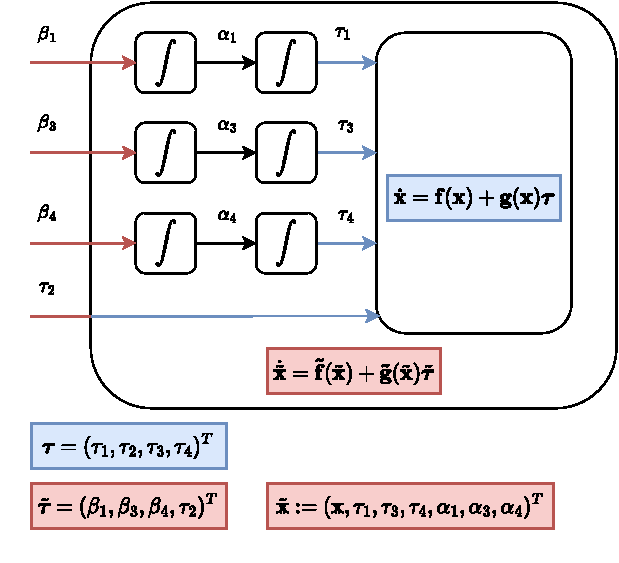
\includegraphics[width=72mm]{images/dynamic_extension}
	}
	\end{textblock*}
	
	\begin{textblock*}{72mm}[0.,0.](90mm,13mm)
	\visible<1->{
		\begin{itemize}
			\item Vorschalten von Integratoren vor $\boldsymbol{\tau}$:
			\begin{align*}
				\beta_1 &:= \dot{\alpha}_1 \hspace{1cm} \alpha_1 := \dot{\tau}_1 \\
				\beta_3 &:= \dot{\alpha}_3 \hspace{1cm} \alpha_3 := \dot{\tau}_3 \\
				\beta_4 &:= \dot{\alpha}_4 \hspace{1cm} \alpha_4 := \dot{\tau}_4 
			\end{align*}
		\end{itemize}
	}
	\visible<2->{
		\begin{itemize}	
			\item[$\rightarrow$] Erweiterung des ZRM $\mathbf{\tilde{f}}$, $\mathbf{\tilde{g}}$ mit $\tilde{\boldsymbol{\tau}}$, $\tilde{\mathbf{x}}$
			\item[$\rightarrow$] $r_i = 4$ für $i = 1, \hdots, 4$
		\end{itemize}
	}
	\visible<3->{
		\begin{itemize}
			\item[$\rightarrow$] neue Entkokkplungsmatrix ($* \neq 0$):
			\begin{align*}
				\tilde{\boldsymbol{\Lambda}} =
				\left(\begin{matrix}
					0 & * & * & * \\
					0 & * & * & * \\
					0 & * & * & * \\
					* & * & 0 & 0 \\
				\end{matrix}\right)
				\Rightarrow \text{regulär!}
			\end{align*}
		\end{itemize}
	}
	\end{textblock*}
	
\end{frame}

%%%%%%%%%%%%%%%%%%%%%%%%%%%%%%%%%%%%%%%%%%%%%%%%%%%%%%%%%%%%

\begin{frame}[t,fragile,label=trajektorienregelung_6]{\large Trajektorienfolgeregelung - \textcolor{blue}{Dynamische} \textcolor{red}{Rückführung}}
	
	\begin{itemize}
		\item mit $\tilde{\bullet}$~-Größen nun Entkopplung und Stabilisierung analog statischer Rückführung:
		\begin{align*}
			\tilde{\boldsymbol{\tau}} = \mathbf{u} = \tilde{\boldsymbol{\Lambda }}^{-1}(\mathbf{x}) \cdot (\mathbf{v} - \tilde{\boldsymbol{\Gamma}}(\mathbf{x}))
		\end{align*}
		\pause
		\item funktionale Zusammenhänge der Folgeregelung:
		\begin{align*}
			\textcolor{blue}{\beta_1} &= \mathrm{func}(\mathbf{x}, \textcolor{red}{\tau_1, \tau_3, \tau_4, \alpha_1, \alpha_3, \alpha_4}, \mathbf{y}_{\mathrm{ref}}, \dot{\mathbf{y}}_{\mathrm{ref}}, \ddot{\mathbf{y}}_{\mathrm{ref}}, \mathbf{y}_{\mathrm{ref}}^{(3)}, \mathbf{y}_{\mathrm{ref}}^{(4)}) \\
			\textcolor{blue}{\beta_3} &= \mathrm{func}(\mathbf{x}, \textcolor{red}{\tau_1, \tau_3, \tau_4, \alpha_3, \alpha_4}, \mathbf{y}_{\mathrm{ref}}, \dot{\mathbf{y}}_{\mathrm{ref}}, \ddot{\mathbf{y}}_{\mathrm{ref}}, \mathbf{y}_{\mathrm{ref}}^{(3)}, \mathbf{y}_{\mathrm{ref}}^{(4)}) \\
			\textcolor{blue}{\beta_4} &= \mathrm{func}(\mathbf{x}, \textcolor{red}{\tau_1, \tau_3, \tau_4, \alpha_3, \alpha_4}, \mathbf{y}_{\mathrm{ref}}, \dot{\mathbf{y}}_{\mathrm{ref}}, \ddot{\mathbf{y}}_{\mathrm{ref}}, \mathbf{y}_{\mathrm{ref}}^{(3)}, \mathbf{y}_{\mathrm{ref}}^{(4)}) \\
			\tau_2 &= \mathrm{func}(\mathbf{x}, \tau_1, \tau_3, \tau_4, \alpha_3, \alpha_4, \mathbf{y}_{\mathrm{ref}}, \dot{\mathbf{y}}_{\mathrm{ref}}, \ddot{\mathbf{y}}_{\mathrm{ref}}, \mathbf{y}_{\mathrm{ref}}^{(3)}, \mathbf{y}_{\mathrm{ref}}^{(4)})
		\end{align*}
		\pause
		\item Anpassung der Trajektorienplanung, da Vorgabe von $\beta_i$ (Doppelintegratoren)
		\pause
		\item[$\rightarrow$] für alle $y_i$ nun 5 Bedingungen je Rand
		\item[$\rightarrow$] Ansatz von Polynomen der Ordnung 9
	\end{itemize}
	
\end{frame}

%%%%%%%%%%%%%%%%%%%%%%%%%%%%%%%%%%%%%%%%%%%%%%%%%%%%%%%%%%%%

\begin{frame}[t,fragile,label=trajektorienregelung_71]{\large Trajektorienfolgeregelung - Dynamische Rückführung}
	
	\textbf{Simulation:}
	\begin{center}
		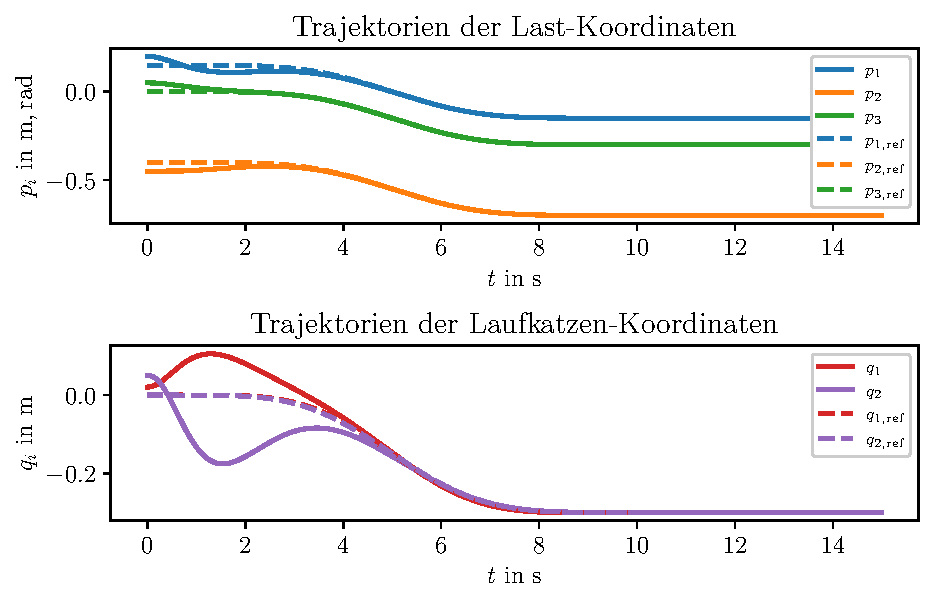
\includegraphics[width=95mm]{images/dyn_controller_initial_error_flat_output}
	\end{center}
	
\end{frame}

%%%%%%%%%%%%%%%%%%%%%%%%%%%%%%%%%%%%%%%%%%%%%%%%%%%%%%%%%%%%

\begin{frame}[t,fragile,label=trajektorienregelung_72]{\large Trajektorienfolgeregelung - Dynamische Rückführung}
	
	\textbf{Simulation:}
	\begin{center}
		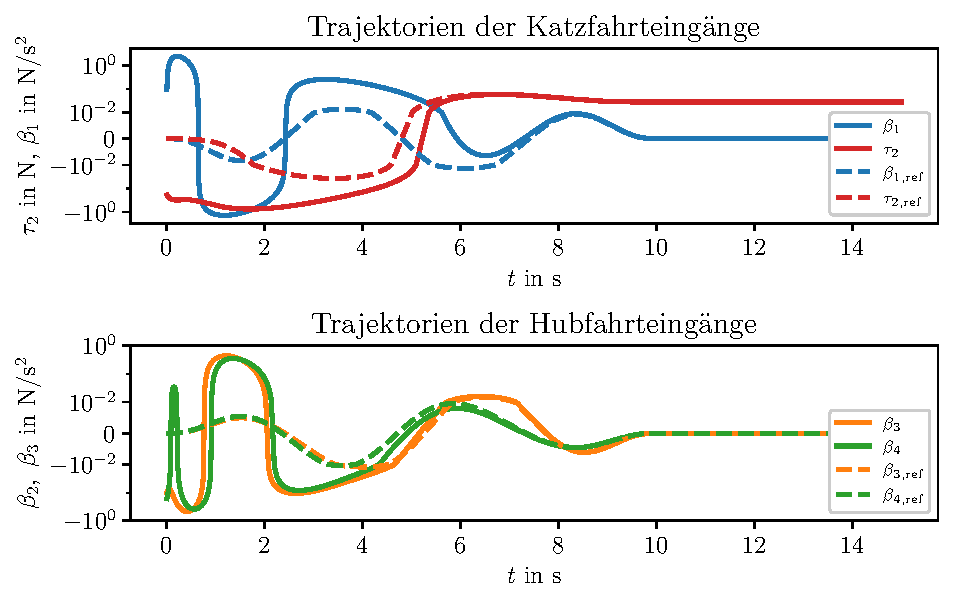
\includegraphics[width=95mm]{images/dyn_controller_initial_error_inputs}
	\end{center}
	
\end{frame}

%%%%%%%%%%%%%%%%%%%%%%%%%%%%%%%%%%%%%%%%%%%%%%%%%%%%%%%%%%%%

\begin{frame}[t,fragile,label=trajektorienregelung_8]{\large Trajektorienfolgeregelung - Dynamische Rückführung}
	
	\textbf{Fazit:}
	\begin{itemize}
		\item akkurate Trajektorienfolge und stationäre Genauigkeit auch bei Anfangsfehlern
		\bigskip
		\pause
		\item hohe „Trägheit“ des Systems beim Ausregeln von Folgefehlern wegen Integratoren
		\item[$\rightarrow$] Pole der Fehlerdynamik weiter in LHE platzieren
		\bigskip
		\pause
		\item relativ komplexes Stellgesetz mit >20\,000 Operationen je Eingangsgröße
		\item[$\rightarrow$] lange Simulationszeiten, hohe Ressourcenanforderungen bei Implementierungen
		\pause
		\item[$\rightarrow$] vereinfachter heuristischer Ansatz mit \textbf{exact feedforward linearization}
	\end{itemize}
	
\end{frame}
 
%%%%%%%%%%%%%%%%%%%%%%%%%%%%%%%%%%%%%%%%%%%%%%%%%%%%%%%%%%%%

\begin{frame}[t,fragile,label=trajektorienregelung_9]{\large Trajektorienfolgeregelung - Exact feedforward linearization}
	
	\begin{itemize}
		\item bisher Rückführung nach Prinzip der exakten Eingangs-Ausgangs-Linearisierung:
		\begin{align*}
			\mathbf{u} = \boldsymbol{\Lambda }^{-1}(\mathbf{x}) \cdot (\mathbf{v} - \boldsymbol{\Gamma}(\mathbf{x}))
		\end{align*}
		\item[$\rightarrow$] nun exact \textcolor{red}{feedforward} linearization:
		\begin{align*}
			\mathbf{u} = \boldsymbol{\Lambda}^{-1}(\mathbf{x}_{\textcolor{red}{\text{ref}}}) \cdot (\mathbf{v} - \boldsymbol{\Gamma}(\mathbf{x}_{\textcolor{red}{\text{ref}}}))
		\end{align*}
		\pause
		\item aus ZRM $\dot{\mathbf{x}} = \mathbf{f}(\mathbf{x}) + \mathbf{g}(\mathbf{x}) \ \mathbf{u}$ mit $\mathbf{x} = (\boldsymbol{\theta}, \dot{\boldsymbol{\theta}})^T$:
		\begin{align*}
			\ddot{\boldsymbol{\theta}} = \mathbf{f}_{\textcolor{blue}{[6, 10]}}(\boldsymbol{\theta}) + \mathbf{g}_{\textcolor{blue}{[6, 10]}}(\boldsymbol{\theta}) \ \mathbf{u}
		\end{align*}
		\pause
		\item[$\rightarrow$] \textbf{Heuristik}: Entkopplungsmatrix $\boldsymbol{\Lambda}(\mathbf{x}_{\text{ref}}) = \mathbf{g}_{[6, 10]}(\boldsymbol{\theta_{\text{ref}}})$
		\pause
		\item[$\rightarrow$] \textbf{Heuristik}: Annahme der Dynamik der \textbf{Ordnung 2} des Fehlers $\mathbf{e} := \boldsymbol{\theta} - \boldsymbol{\theta}_{\text{ref}}$ für \textbf{alle} Komponenten des Koordinatenvektors $\boldsymbol{\theta} = (p_1, p_2, p_3, q_1, q_2)^T$
		\pause
		\item[$\rightarrow$] Pseudoinverse für $\boldsymbol{\Lambda}^{-1}$ nötig, da $\mathbf{g}_{[6, 10]} \in \mathbb{R}^{5 \times 4}$
		
	\end{itemize}
	
	\begin{textblock*}{50mm}[0.,0.](108mm, 18mm)
		\visible<2-2>{
			\begin{tcolorbox}[colback=lightgray,colframe=softblue,title=Brückenkransystem]
				$\mathbf{f}(\mathbf{x}) = 
				(\dot{\boldsymbol{\theta}}, \textcolor{blue}{0}, \textcolor{blue}{-g}, \textcolor{blue}{0}, \textcolor{blue}{0}, \textcolor{blue}{0})^T$, \\ 
				$\mathbf{g}(\mathbf{x}) =
				\left(\begin{matrix}
					0 & 0 & 0 & 0\\
					0 & 0 & 0 & 0\\
					0 & 0 & 0 & 0\\
					0 & 0 & 0 & 0\\
					0 & 0 & 0 & 0\\
					\textcolor{blue}{0} & \textcolor{blue}{0} & \textcolor{blue}{*} & \textcolor{blue}{*}\\
					\textcolor{blue}{0} & \textcolor{blue}{0} & \textcolor{blue}{*} & \textcolor{blue}{*}\\
					\textcolor{blue}{0} & \textcolor{blue}{0} & \textcolor{blue}{*} & \textcolor{blue}{*}\\
					\textcolor{blue}{*} & \textcolor{blue}{0} & \textcolor{blue}{*} & \textcolor{blue}{0}\\
					\textcolor{blue}{0} & \textcolor{blue}{*} & \textcolor{blue}{0} & \textcolor{blue}{*}
				\end{matrix}\right)$
			\end{tcolorbox}
		}
	\end{textblock*}
	
\end{frame}

%%%%%%%%%%%%%%%%%%%%%%%%%%%%%%%%%%%%%%%%%%%%%%%%%%%%%%%%%%%%

\begin{frame}[t,fragile,label=trajektorienregelung_121]{\large Trajektorienfolgeregelung - Exact feedforward linearization}
	
	\textbf{Simulation:}
	\begin{center}
		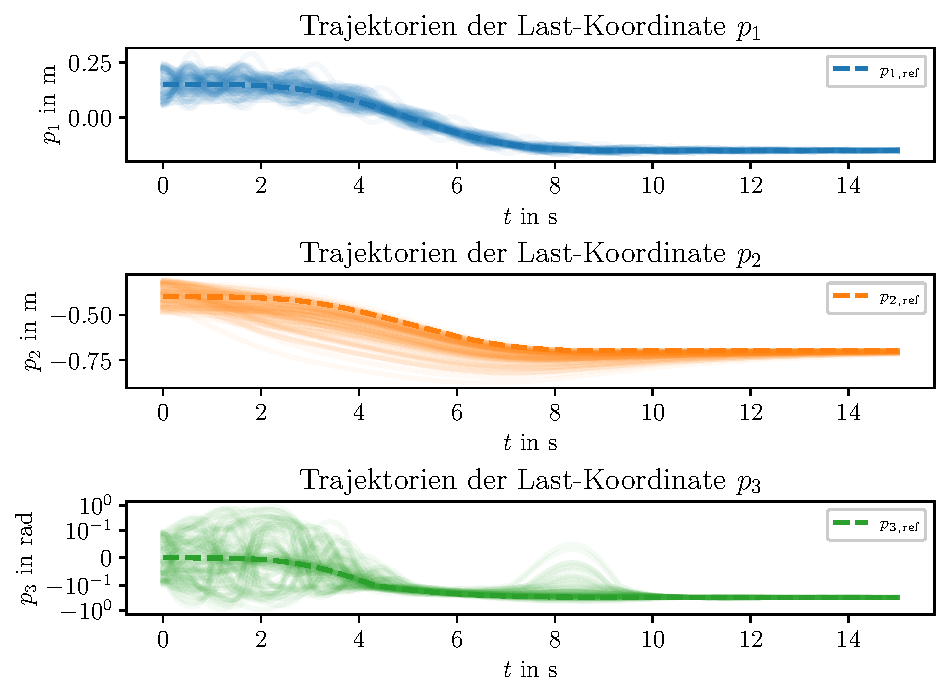
\includegraphics[width=85mm]{images/feedforward_lin_selection_initial_error_ensemble_flat_output}
	\end{center}

\end{frame}

%%%%%%%%%%%%%%%%%%%%%%%%%%%%%%%%%%%%%%%%%%%%%%%%%%%%%%%%%%%%

\begin{frame}[t,fragile,label=trajektorienregelung_122]{\large Trajektorienfolgeregelung - Exact feedforward linearization}
	
	\textbf{Simulation:}
	\begin{center}
		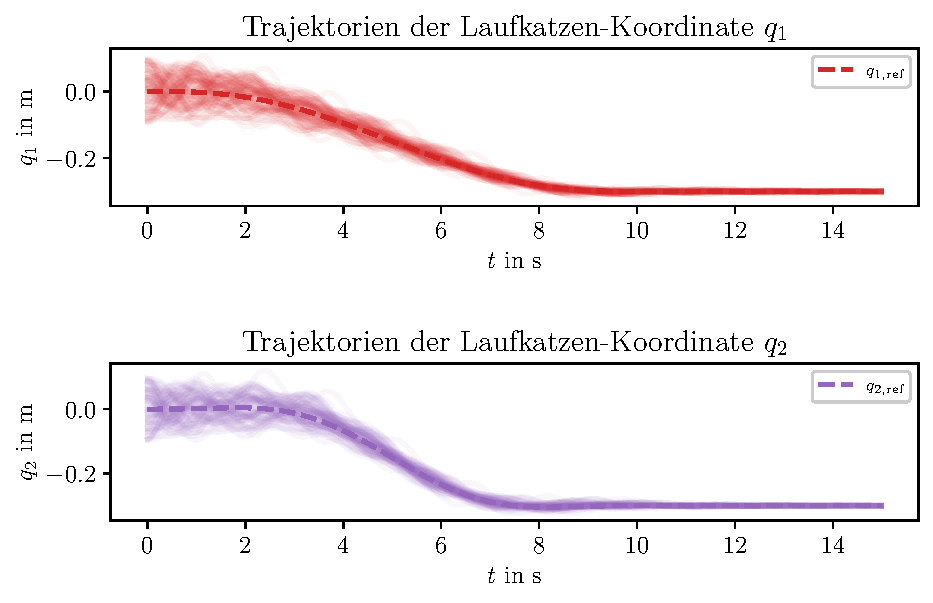
\includegraphics[width=95mm]{images/feedforward_lin_selection_initial_error_ensemble_flat_output_q}
	\end{center}
	
\end{frame}

%%%%%%%%%%%%%%%%%%%%%%%%%%%%%%%%%%%%%%%%%%%%%%%%%%%%%%%%%%%%

\begin{frame}[t,fragile,label=trajektorienregelung_13]{\large Trajektorienfolgeregelung - Exact feedforward linearization}
	
	\textbf{Fazit:}
	\begin{itemize}
		\item akkurate Trajektorienfolge und stationäre Genauigkeit auch bei Anfangsfehlern
		\bigskip
		\pause
		\item kein Stabilitätsnachweis für zeitvariantes System, aber auch kein Gegenbeispiel aus Ensemble-Simulation
		\pause
		\bigskip
		\item Stellgesetz mit weniger als 140 Operationen je Eingangskomponente
		\item[$\rightarrow$] viel kürzere Simulationszeiten, geringere Ressourcenanforderungen für Implementierung
	\end{itemize}

\end{frame}

%%%%%%%%%%%%%%%%%%%%%%%%%%%%%%%%%%%%%%%%%%%%%%%%%%%%%%%%%%%%

\begin{frame}<1>[label=gl5]
	\frametitle{Gliederung}
	\begin{itemize}
		%0
		\item[\cdbox] System- und Problembeschreibung
		%1
		\item[\cdbox] Analytische Modellbildung
		%2
		\item[\cdbox] Flachheitsanalyse
		%3
		\item[\cdbox] Steuerungs- und Regelungsentwurf
		%4
		\item[\only<1>{$\rightarrow$}\only<2>{$\rightarrow$}\only<4->{\cdbox}]
		\textbf<1>{Zusammenfassung und Ausblick}
	\end{itemize}
\end{frame}

%%%%%%%%%%%%%%%%%%%%%%%%%%%%%%%%%%%%%%%%%%%%%%%%%%%%%%%%%%%%

\begin{frame}[label=Zusammenfassung1]
	\frametitle{Zusammenfassung {\color<1->{mygray}und Ausblick}}
	\begin{itemize}
		\item Modellierung des Brückenkrans als nichtlineares Mehrgrößensystem in ODE-Form durch LG2
		\item[$\rightarrow$] gute Eignung für Simulation und Flachheitsanalyse
		\bigskip
		\pause
		\item Flachheitsanalyse und Ermittlung eines flachen Ausgangs $\mathbf{y}$ für das Doppelkransystem mit CAS SymPy
		\bigskip
		\pause
		\item Planung polynombasierter Trajektorien für $\mathbf{y}$ zur Ruhelagenüberführung
		\item[$\rightarrow$] Steuerung aus Parametrisierung des Eingangs $\boldsymbol{\tau}(\mathbf{y}, \dot{\mathbf{y}})$
		
	\end{itemize}
	
\end{frame}

%%%%%%%%%%%%%%%%%%%%%%%%%%%%%%%%%%%%%%%%%%%%%%%%%%%%%%%%%%%%

\begin{frame}[label=Zusammenfassung2]
	\frametitle{Zusammenfassung {\color<1->{mygray}und Ausblick}}
	\begin{itemize}
		\item Regelung durch statische Rückführung nicht möglich
		\item[$\rightarrow$] Entkopplungsmatrix $\boldsymbol{\Lambda}$ nicht invertierbar
		\pause
		\item dynamische Erweiterung mit linearer Fehlerdynamik
		\item[$\rightarrow$] per Konstruktion stabil, allerdings relativ komplexes Stellgesetz
		\pause
		\item[$\rightarrow$] weiterer heuristischer Ansatz zur Vereinfachung
		\pause
		\item exact feedforward linearization mit Fehlerdynamik 2ter Ordnung in allen Koordinaten
		\item[$\rightarrow$] relativ kompaktes Stellgesetz, Stabilität nur durch Ensemble-Simulationen untersucht
		
	\end{itemize}
	
\end{frame}

%%%%%%%%%%%%%%%%%%%%%%%%%%%%%%%%%%%%%%%%%%%%%%%%%%%%%%%%%%%%

\begin{frame}[label=Ausblick]
	\frametitle{Zusammenfassung und Ausblick}
	\begin{itemize}
		\item Implementierung auf Demonstratorsystem unter realen Echtzeitanforderungen
		\pause
		\item Test reiner Vorsteuerung und Abschätzung der Größe der Modellabweichung
		\pause
		\item[$\rightarrow$] danach Regelungsansätze unter Stellgrößenbeschränkung und Überwachung der Stabilität
		\pause 
		\item Stabilitätsuntersuchung der exact feedforward linearization als zeitvariantes System
		\pause
		\item bestärkendes Lernen als weiterer Ansatz ggf. mit Referenzlernen auf Basis bisheriger Regelungen
		\pause
		\item Untersuchung der Robustheit gegenüber Modellabweichungen, Störeingriffen
		
	\end{itemize}
	
\end{frame}

%%%%%%%%%%%%%%%%%%%%%%%%%%%%%%%%%%%%%%%%%%%%%%%%%%%%%%%%%%%%

\begin{frame}[fragile,label=Ergaenzungsfolien]{~}
	\begin{center}
		{\huge \textbf{Ergänzungsfolien}} 
	\end{center}
	
\end{frame}

\backupbegin

%%%%%%%%%%%%%%%%%%%%%%%%%%%%%%%%%%%%%%%%%%%%%%%%%%%%%%%%%%%%%%%%%%%%%%%%%%%%%%%%

\begin{frame}[t,fragile,label=Lagrange2_1]{\large Lagrange-Formalismus}
	
	\textbf{Symbole:}
	\begin{itemize}
		\item Konfigurationskoordinaten $\boldsymbol{\theta} = (\mathbf{q}, \mathbf{p})^T$
		\pause
		\item direkt aktuierte Koordinaten $\mathbf{q}$, nicht direkt aktuierte Koordinaten $\mathbf{p}$
		\pause
		\item kinetische Energie $T(\boldsymbol{\theta}, \dot{\boldsymbol{\theta}})$, potentielle Energie $V(\boldsymbol{\theta})$
		\pause
		\item Lagrange-Funktion $\mathcal{L}(\boldsymbol{\theta}, \dot{\boldsymbol{\theta}}) = T(\boldsymbol{\theta}, \dot{\boldsymbol{\theta}}) - V(\boldsymbol{\theta})$
		\pause
		\item verallgemeinerte Kraft $\mathbf{Q} = \mathbf{f} - \mathbf{D}$
		\pause
		\item äußere Stellkraft $\mathbf{f}$, interne Reibungskraft $\mathbf{D}$
	\end{itemize}
	
	\pause
	\bigskip
	\textbf{Lagrange-Gleichungen zweiter Art:}
	\begin{itemize}
		\pause
		\item  $\boldsymbol{\theta}$ sind unabhängig (ohne Zwangsbedingung verkoppelt)
		\pause
		\item Bewegungsgleichungen:
		\begin{equation*}
			\frac{\mathrm{d}}{\mathrm{d} t} \left(\frac{\partial \mathcal{L}}{\partial \dot{\theta}_i} \right) - \frac{\partial \mathcal{L}}{\partial \theta_i} = Q_i, \quad i = 1, \ldots, n
		\end{equation*}
		\pause
		\item Woher $Q_i$?
	\end{itemize}
	
\end{frame}

%%%%%%%%%%%%%%%%%%%%%%%%%%%%%%%%%%%%%%%%%%%%%%%%%%%%%%%%%%%%

\begin{frame}[t,fragile,label=Lagrange2_2]{\large Lagrange-Formalismus}
	
	\textbf{Symbole:}
	\begin{itemize}
		\item Konfigurationskoordinaten $\boldsymbol{\theta} = (\mathbf{q}, \mathbf{p})^T$
		\item verallgemeinerte Kraft $\mathbf{Q} = \mathbf{f} - \mathbf{D}$
		\pause
		\item Richtungsvektor zu $k$-tem massebehaftetem Partikel $\mathbf{r}_k$, Stellkraft $\mathbf{F}_k$ entlang $\mathbf{r}_k$
		\pause
		\item virtuelle Arbeit $\delta W$, virtuelle Verschiebung von Partikel $\delta \mathbf{r}_k$ und Koordinate $\theta_{i}$
	\end{itemize}
	
	\pause
	\bigskip
	\textbf{Prinzip der virtuellen Arbeit zur Bestimmung der $Q_i$:}
	\begin{itemize}
		\pause
		\item  $\delta W = \sum_{k=1}^l \mathbf{F}_k \cdot \frac{\partial \mathbf{r}_k}{\partial \theta_1} \delta \theta_1 +\ldots + \sum_{k=1}^l \mathbf{F}_k \cdot \frac{\partial \mathbf{r}_k}{\partial \theta_n} \delta \theta_n$
		\pause
		\item $\delta \mathbf{r}_{k} = \sum_{i = 1}^{n} \frac{\partial\mathbf{r}_{k}}{\partial\theta_i} \delta \theta_i$
		\pause
		\item $\delta W = \sum_{k=1}^{l}\delta \mathbf{r}_k^T \mathbf{F}_k = Q_1 \delta \theta_1 + \ldots + Q_n\delta \theta_n$
		\pause
		\item[$\rightarrow$] $Q_i = \sum_{k=1}^l \left(\frac {\partial \mathbf{r_k}} {\partial \theta_i} \right)^T \mathbf {F}_{k} = \frac{\partial\delta W}{\partial \delta \theta_i} ,\quad i=1,\ldots, n$
	\end{itemize}
	
\end{frame}

%%%%%%%%%%%%%%%%%%%%%%%%%%%%%%%%%%%%%%%%%%%%%%%%%%%%%%%%%%%%

\begin{frame}[t,fragile,label=ModellEinzelkran_1]{\large Analytisches Modell Einzelkran}
	\begin{textblock*}{80mm}[0.,0.](12mm,13mm)	
		\visible<1->{
			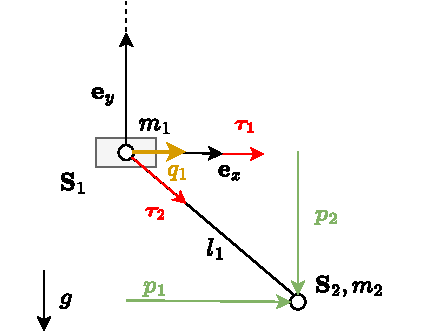
\includegraphics[width=64mm]{images/ODE_flatness_analysis_single_crane_diagram}
		}
		\bigskip
		\visible<2->{
			\begin{itemize}
				\item Massen bei $\mathbf{S}_1 = (q_1, 0)^T$, $\mathbf{S}_2 = (p_1, p_2)^T$
				\item variable Seillänge $l_1 = \sqrt{(p_1 - q_1)^2 + p_2^2}$\\
				~
			\end{itemize}
		}
	\end{textblock*}
	
	\begin{textblock*}{80mm}[0.,0.](80mm,13mm)
		
		\visible<3->{	
			\textbf{Energien:}			
			\begin{itemize}
				\item $T = \frac{m_1}{2} \dot{\mathbf{S}}_1^T \dot{\mathbf{S}}_1 + \frac{m_2}{2} \dot{\mathbf{S}}_2^T \dot{\mathbf{S}}_2 = \frac{m_{1} \dot{q}_{1}^{2}}{2} + \frac{m_{2} \dot{p}_{1}^{2}}{2} + \frac{m_{2} \dot{p}_{2}^{2}}{2}$
				\item $V = m_2 g \ \mathbf{S}_2^T \mathbf{e}_y = m_{2} g p_{2}$
			\end{itemize}
		}
		
	\end{textblock*}
	
	\begin{textblock*}{80mm}[0.,0.](80mm,35mm)
		
		\visible<4->{
			\textbf{Verallgemeinerte Kraft aus virtueller Arbeit:}
			\begin{itemize}
				\item $\mathbf{F}_1 =
				\left(\tau_{1}, 0 \right)^T$,
				$\mathbf{F}_2 =
				\left(\frac{\tau_{2} \left(p_{1} - q_{1}\right)}{l_{1}}, \frac{p_{2} \tau_{2}}{l_{1}} \right)^T$
				\item[$\rightarrow$] $\mathbf{Q} = \left(\frac{\tau_{2} \left(p_{1} - q_{1}\right)}{l_{1}}, \frac{p_{2} \tau_{2}}{l_{1}}, \tau_{1} - \frac{\tau_{2} \left(p_{1} - q_{1}\right)}{l_{1}} \right)^T$
			\end{itemize}
		}
		
	\end{textblock*}
	
\end{frame}

%%%%%%%%%%%%%%%%%%%%%%%%%%%%%%%%%%%%%%%%%%%%%%%%%%%%%%%%%%%%

\begin{frame}[t,fragile,label=ModellDoppelkran_1]{\large Analytisches Modell Doppelkran}
	\begin{textblock*}{80mm}[0.,0.](12mm,13mm)	
		\visible<1->{
			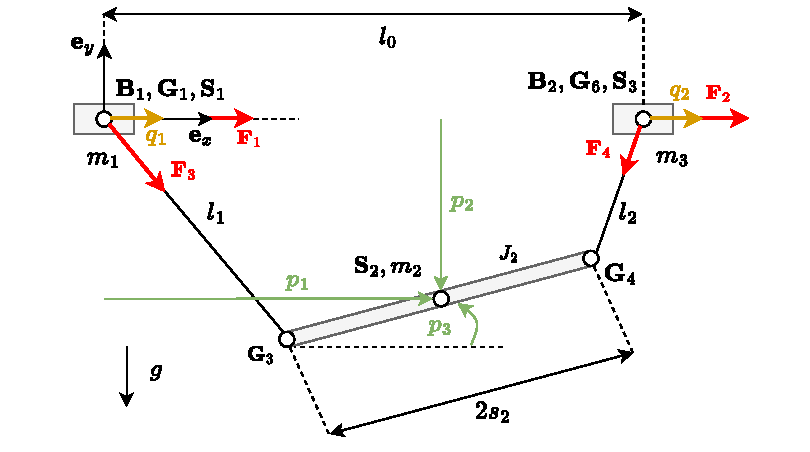
\includegraphics[width=64mm]{images/ODE_flatness_analysis_double_crane_diagram}
		}
		\bigskip
		\visible<2->{
			\textbf{variable Seillängen:}
			\tiny{
				\begin{flalign*}
					l_1 &= \sqrt{\left(p_{2} - s_{2} \sin{\left(p_{3} \right)}\right)^{2} + \left(p_{1} - q_{1} - s_{2} \cos{\left(p_{3} \right)}\right)^{2}}&& \\
					l_2 &= \sqrt{\left(p_{2} + s_{2} \sin{\left(p_{3} \right)}\right)^{2} + \left(- l_{0} + p_{1} - q_{2} + s_{2} \cos{\left(p_{3} \right)}\right)^{2}}&&
				\end{flalign*}
			}
			~
		}
	\end{textblock*}
	
	\begin{textblock*}{80mm}[0.,0.](80mm,13mm)
		
		\visible<3->{	
			\textbf{Energien:}			
			\begin{itemize}
				\item $T = \frac{J_{2} \dot{p}_{3}^{2}}{2} + \frac{m_{1} \dot{q}_{1}^{2}}{2} + \frac{m_{2} \dot{p}_{1}^{2}}{2} + \frac{m_{2} \dot{p}_{2}^{2}}{2} + \frac{m_{3} \dot{q}_{2}^{2}}{2}$
				\item $V =m_{2} g p_{2}$
			\end{itemize}
		}
	\end{textblock*}
	
	\begin{textblock*}{80mm}[0.,0.](80mm,35mm)
		
		\visible<4->{
			\textbf{Stellkräfte entlang Massepartikel:}
			\begin{flalign*}
				\mathbf{F}_1 &=
				\left( \tau_{1}, 0 \right)^T, \\
				\mathbf{F}_2 &=
				\left( \tau_{2}, 0 \right)^T, \\
				\mathbf{F}_3 &=
				\left(\begin{matrix}
					\frac{\tau_{3} \left(p_{1} - q_{1} - s_{2} \cos{\left(p_{3} \right)}\right)}{l_{1}}\\
					\frac{\tau_{3} \left(p_{2} - s_{2} \sin{\left(p_{3} \right)}\right)}{l_{1}}
				\end{matrix}\right), \\
				\mathbf{F}_4 &=
				\left(\begin{matrix}
					\frac{\tau_{4} \left(- l_{0} + p_{1} - q_{2} + s_{2} \cos{\left(p_{3} \right)}\right)}{l_{2}}\\
					\frac{\tau_{4} \left(p_{2} + s_{2} \sin{\left(p_{3} \right)}\right)}{l_{2}}
				\end{matrix}\right)
			\end{flalign*}
		}
		
	\end{textblock*}
	
\end{frame}

%%%%%%%%%%%%%%%%%%%%%%%%%%%%%%%%%%%%%%%%%%%%%%%%%%%%%%%%%%%%

\begin{frame}[t,fragile,label=Flachheit_3]{\large Flachheitsanalyse von MIMO-Systemen}
	
	\textbf{Elimination von Systemgrößen- und Gleichungen:}
	
	\begin{itemize}
		\pause
		\item Jacobi-Matrix $\mathbf{J}_i$ der $i$ bisher nicht eliminierter Systemgleichungen bezüglich nicht eliminierter Eingangskomponenten $\mathbf{u}_{m-(n-i)}$ (später analog für $\mathbf{x}_{i+m}$): \\
		\pause
		\begin{equation*}
			\mathbf{J}_i = 
			\begin{pmatrix}
				* & \cdots & * & 0 & * & \cdots & *\\
				\vdots & \ddots & \vdots & \vdots & \vdots & \ddots & \vdots \\
				* & \cdots & * & 0 & * & \cdots & *  \\
				* & \cdots & * & \varepsilon & * & \cdots & * \\
				* & \cdots & * & 0 & * & \cdots & *  \\
				\vdots & \ddots & \vdots & \vdots & \vdots & \ddots & \vdots \\
				* & \cdots & * & 0 & * & \cdots & *\\
			\end{pmatrix}
		\end{equation*}
		\pause
		\item[$\rightarrow$] Identifikation einer Spalte mit nur einem nicht-Null-Eintrag
		\pause
		\item[$\rightarrow$] Elimination der mit Spalte korrespondierenden Eingangskomponente und Zeile korrespondierender Gleichung
	\end{itemize}
	
\end{frame}

%%%%%%%%%%%%%%%%%%%%%%%%%%%%%%%%%%%%%%%%%%%%%%%%%%%%%%%%%%%%

\begin{frame}[t,fragile,label=Flachheit_4]{\large Flachheitsanalyse von MIMO-Systemen}
	
	\textbf{Elimination von Systemgrößen- und Gleichungen:}
	
	\begin{itemize}
		\item  Wie vorgehen, wenn keine solche Spalte auffindbar?
		\pause
		\item[$\rightarrow$] Transformation der Systemgleichungen mit Matrix $\mathbf{T}_i$: \\
		\begin{equation*}
			\mathbf{T}_i \mathbf{J}_i = 
			\begin{pmatrix}
				\mathbf{I}_{m-(n-i)} \\
				\hline
				\mathbf{0}_{(n-m) \times (m-(n-i))}
			\end{pmatrix}
			=
			\begin{pmatrix}
				1 & 0 & \cdots & 0 & 0 \\
				0 & 1 & \cdots & 0 & 0 \\
				\vdots & & \ddots &  & \vdots \\
				0 & 0 & \cdots & 1 & 0 \\
				0 & 0 & \cdots & 0 & 1 \\
				\hline
				0 & 0 & \cdots & 0 & 0
			\end{pmatrix}
		\end{equation*}
		\pause
		\item[$\rightarrow$] Konstruktion von $\mathbf{T}_i$ aus linkem Orthokomplement $\mathbf{J}_i^{\mathrm{L} \perp}$ und Pseudoinverser $\mathbf{J}_i^{\mathrm{L} +}$: \\
		\begin{equation*}
			\mathbf{J}_i^{\mathrm{L} +} \mathbf{J}_i = \mathbf{I}_{m-(n-i)}, \quad
			\mathbf{J}_i^{\mathrm{L} \perp} \mathbf{J}_i = \mathbf{0}_{(n-m) \times (m-(n-i))} \quad
			\Rightarrow \mathbf{T}_i = 
			\begin{pmatrix}
				\mathbf{J}_i^{\mathrm{L} +} \\
				\mathbf{J}_i^{\mathrm{L} \perp}
			\end{pmatrix}
		\end{equation*}
	\end{itemize}
	
\end{frame}

%%%%%%%%%%%%%%%%%%%%%%%%%%%%%%%%%%%%%%%%%%%%%%%%%%%%%%%%%%%%

\begin{frame}[t,fragile,label=Flachheit_Einzelkran_1]{\large Flachheitsanalyse am Einzelkran}
	
	\textbf{Elimination von Systemgrößen- und Gleichungen:}
	
	\begin{itemize}
		\item {($i = 3$) Systemgleichungen und Jacobi-Matrix bezüglich $\mathbf{u}_2 = (\tau_1, \tau_2)^T$:}
		\begin{align*}
		\begin{split}
		m_{2} \ddot{p}_{1} - \frac{\tau_{2} \left(p_{1} - q_{1}\right)}{l_{1}} &= 0\\
		g m_{2} + m_{2} \ddot{p}_{2} - \frac{p_{2} \tau_{2}}{l_{1}} &= 0\\
		m_{1} \ddot{q}_{1} - \tau_{1} + \frac{\tau_{2} \left(p_{1} - q_{1}\right)}{l_{1}} &= 0
		\end{split}
		\quad \Rightarrow \quad 
		\mathbf{J}_3 = 
		\left(\begin{matrix}
		0 & - \frac{p_{1} - q_{1}}{\sqrt{p_{2}^{2} + \left(p_{1} - q_{1}\right)^{2}}}\\
		0 & - \frac{p_{2}}{\sqrt{p_{2}^{2} + \left(p_{1} - q_{1}\right)^{2}}}\\
		-1 & \frac{p_{1} - q_{1}}{\sqrt{p_{2}^{2} + \left(p_{1} - q_{1}\right)^{2}}}
		\end{matrix}\right)
		\end{align*}
		\pause
		\item[$\rightarrow$] Elimination von $\tau_1$ und letzter Gleichung	
	\end{itemize}
	
\end{frame}

%%%%%%%%%%%%%%%%%%%%%%%%%%%%%%%%%%%%%%%%%%%%%%%%%%%%%%%%%%%%

\begin{frame}[t,fragile,label=Flachheit_Einzelkran_2]{\large Flachheitsanalyse am Einzelkran}
	
	\textbf{Elimination von Systemgrößen- und Gleichungen:}
	
	\begin{itemize}
		\item {($i = 2$) Systemgleichungen und Jacobi-Matrix bezüglich $\mathbf{u}_1 = \tau_2$:}
		\begin{align*}
		\begin{split}
		m_{2} \ddot{p}_{1} - \frac{\tau_{2} \left(p_{1} - q_{1}\right)}{l_{1}} &= 0\\
		g m_{2} + m_{2} \ddot{p}_{2} - \frac{p_{2} \tau_{2}}{l_{1}} &= 0
		\end{split}
		\quad \Rightarrow \quad 
		\mathbf{J}_2 = 
		\left(\begin{matrix}
		- \frac{p_{1} - q_{1}}{\sqrt{p_{2}^{2} + \left(p_{1} - q_{1}\right)^{2}}}\\
		- \frac{p_{2}}{\sqrt{p_{2}^{2} + \left(p_{1} - q_{1}\right)^{2}}}
		\end{matrix}\right)
		\end{align*}		
		\pause
		\item[$\rightarrow$] keine Spalte mit nur einem nicht-Null-Eintrag, also Transformation $\mathbf{T}_2$ nötig:
		\begin{align*}
		\mathbf{J}_2^{\mathrm{L}+} &=
		\left(
		\left(\begin{matrix}
		J_{2, (1,1)}
		\end{matrix}\right)^{-1}	
		\mathbf{0}_{1 \times 1}
		\right), 		
		\mathbf{J}_2^{\mathrm{L}\perp} =
		\left(\begin{matrix}
		-J_{2, (2,1)} & J_{2, (1,1)}
		\end{matrix}\right) \\
		\Rightarrow
		\mathbf{T}_2 &=
		\left(\begin{matrix}
		\frac{\sqrt{p_{1}^{2} - 2 p_{1} q_{1} + p_{2}^{2} + q_{1}^{2}}}{- p_{1} + q_{1}} & 0\\
		\frac{p_{2}}{\sqrt{p_{2}^{2} + \left(p_{1} - q_{1}\right)^{2}}} & \frac{- p_{1} + q_{1}}{\sqrt{p_{2}^{2} + \left(p_{1} - q_{1}\right)^{2}}}
		\end{matrix}\right)
		\end{align*}
		
	\end{itemize}
	
\end{frame}

%%%%%%%%%%%%%%%%%%%%%%%%%%%%%%%%%%%%%%%%%%%%%%%%%%%%%%%%%%%%

\begin{frame}[t,fragile,label=Flachheit_Einzelkran_3]{\large Flachheitsanalyse am Einzelkran}
	
	\textbf{Elimination von Systemgrößen- und Gleichungen:}
	
	\begin{itemize}
		\item {($i = 2$) transformierte Systemgleichungen und Jacobi-Matrix bezüglich $\mathbf{u}_1 = \tau_2$:}
		\begin{align*}
		\begin{split}
		\frac{\left(- m_{2} \ddot{p}_{1} \sqrt{p_{2}^{2} + \left(p_{1} - q_{1}\right)^{2}} + \tau_{2} \left(p_{1} - q_{1}\right)\right)}{\left(p_{1} - q_{1}\right)} &= 0 \label{single_flat_transformed_syseq1}\\
		g\frac{m_{2} \left(- g p_{1} + g q_{1} - p_{1} \ddot{p}_{2} + p_{2} \ddot{p}_{1} + \ddot{p}_{2} q_{1}\right)}{\sqrt{p_{1}^{2} - 2 p_{1} q_{1} + p_{2}^{2} + q_{1}^{2}}}
		&= 0
		\end{split}
		\quad \Rightarrow \quad 
		\mathbf{J}_2' = 
		\left(\begin{matrix}
		1\\
		0
		\end{matrix}\right)
		\end{align*}		
		\pause
		\item[$\rightarrow$] Elimination von $\tau_2$ und erster transformierter Gleichung
		\pause
		\item[$\rightarrow$] letzte übrige Gleichung enthält folgende Menge an Systemgrößen:
		\begin{equation*}
		\mathcal{M} = \{p_1, \ddot{p}_1, p_2, \ddot{p}_2, q_1 \}
		\end{equation*}
		\pause
		\item rein algebraisches Auftreten von $q_1$ führt zu Wahl von $\mathbf{y} = (p_1, p_2)^T$
		
	\end{itemize}
	
\end{frame}

%%%%%%%%%%%%%%%%%%%%%%%%%%%%%%%%%%%%%%%%%%%%%%%%%%%%%%%%%%%%

\begin{frame}[t,fragile,label=Flachheit_Einzelkran_4]{\large Flachheitsanalyse am Einzelkran}
	
	\textbf{Parametisierung der Systemgrößen durch $\mathbf{y} = (p_1, p_2)^T$:}
	
	\begin{itemize}
		\pause
		\item aus letzter transformierter Systemgleichung:
		\begin{equation*}
		q_1 = \frac{g p_{1} + p_{1} \ddot{p}_{2} - p_{2} \ddot{p}_{1}}{g + \ddot{p}_{2}}
		\end{equation*}
		\pause 
		\item aus erster transformierter Systemgleichung und Einsetzen von $q_1(\mathbf{y}, \ddot{\mathbf{y}})$:
		\begin{equation*}
		\tau_2 = \frac{m_{2} \ddot{p}_{1} \sqrt{p_{2}^{2} + \left(p_{1} - \frac{g p_{1} + p_{1} \ddot{p}_{2} - p_{2} \ddot{p}_{1}}{g + \ddot{p}_{2}}\right)^{2}}}{p_{1} - \frac{g p_{1} + p_{1} \ddot{p}_{2} - p_{2} \ddot{p}_{1}}{g + \ddot{p}_{2}}}
		\end{equation*}
	\end{itemize}
	
\end{frame}

%%%%%%%%%%%%%%%%%%%%%%%%%%%%%%%%%%%%%%%%%%%%%%%%%%%%%%%%%%%%

\begin{frame}[t,fragile,label=Flachheit_Einzelkran_5]{\large Flachheitsanalyse am Einzelkran}
	
	\textbf{Parametisierung der Systemgrößen durch $\mathbf{y} = (p_1, p_2)^T$:}
	
	\begin{itemize}
		\item aus zuerst eliminierter originaler Systemgleichung:
		\begin{equation*}
		\tau_1 = \frac{m_{1} \textcolor{red}{\ddot{q}_{1}} \sqrt{p_{2}^{2} + \left(p_{1} - \textcolor{red}{q_{1}}\right)^{2}} + p_{1} \textcolor{red}{\tau_{2}} - \textcolor{red}{q_{1}} \textcolor{red}{\tau_{2}}}{\sqrt{p_{2}^{2} + \left(p_{1} - \textcolor{red}{q_{1}}\right)^{2}}}
		\end{equation*}
		\pause 
		\item[$\rightarrow$] auch Größen $\textcolor{red}{q_1, \ddot{q}_1, \tau_2} \not\in \mathbf{y}$ in dieser Parametrisierung von $\tau_1$ enthalten
		\pause 
		\item[$\rightarrow$] Einsetzen der zweiten Ableitung von $q_1(\mathbf{y}, \ddot{\mathbf{y}})$ und $\tau_2(\mathbf{y}, \ddot{\mathbf{y}})$:
		\begin{flalign*}
		\begin{split}
		\tau_1 &=
		\frac{1}{g^{3} + 3 g^{2} \ddot{p}_{2} + 3 g \ddot{p}_{2}^{2} + \ddot{p}_{2}^{3}}
		(g^{3} m_{1} \ddot{p}_{1} + g^{3} m_{2} \ddot{p}_{1} - g^{2} m_{1} p_{2} \ddddot{p}_{1} - 2 g^{2} m_{1} \dddot{p}_{1} \dot{p}_{2} \\
		&+ 2 g^{2} m_{1} \ddot{p}_{1} \ddot{p}_{2} + 3 g^{2} m_{2} \ddot{p}_{1} \ddot{p}_{2} - 2 g m_{1} p_{2} \ddddot{p}_{1} \ddot{p}_{2} + g m_{1} p_{2} \ddddot{p}_{2} \ddot{p}_{1} + 2 g m_{1} p_{2} \dddot{p}_{1} \dddot{p}_{2} \\
		&- 4 g m_{1} \dddot{p}_{1} \ddot{p}_{2} \dot{p}_{2} + 2 g m_{1} \dddot{p}_{2} \ddot{p}_{1} \dot{p}_{2} + g m_{1} \ddot{p}_{1} \ddot{p}_{2}^{2} + 3 g m_{2} \ddot{p}_{1} \ddot{p}_{2}^{2} - m_{1} p_{2} \ddddot{p}_{1} \ddot{p}_{2}^{2} + m_{1} p_{2} \ddddot{p}_{2} \ddot{p}_{1} \ddot{p}_{2} \\
		& + 2 m_{1} p_{2} \dddot{p}_{1} \dddot{p}_{2} \ddot{p}_{2} - 2 m_{1} p_{2} \dddot{p}_{2}^{2} \ddot{p}_{1} - 2 m_{1} \dddot{p}_{1} \ddot{p}_{2}^{2} \dot{p}_{2} + 2 m_{1} \dddot{p}_{2} \ddot{p}_{1} \ddot{p}_{2} \dot{p}_{2} + m_{2} \ddot{p}_{1} \ddot{p}_{2}^{3})
		\end{split}
		\end{flalign*}
	\end{itemize}
	
\end{frame}

%%%%%%%%%%%%%%%%%%%%%%%%%%%%%%%%%%%%%%%%%%%%%%%%%%%%%%%%%%%%

\begin{frame}[t,fragile,label=Flachheit_Einzelkran_6]{\large Flachheitsanalyse am Einzelkran}
	
	\textbf{Parametisierung der Systemgrößen durch $\mathbf{y} = (p_1, p_2)^T$:}
	
	\begin{itemize}
		\item Zusammenfassung der Parametrisierungen:
		\begin{align*}
		\tau_1 &= \theta_1\left(p_2, \dot{p}_2, \ddot{p}_1, \ddot{p}_2, p_1^{(3)}, p_2^{(3)}, p_1^{(4)}, p_2^{(4)} \right) \\
		\tau_2 &= \theta_2(p_1, p_2, \ddot{p}_1, \ddot{p}_2) \\
		q_1 &= \Psi_1(p_1, p_2, \ddot{p}_1, \ddot{p}_2)
		\end{align*}
		\pause
		\item[$\rightarrow$] alle Systemgrößen durch flachen Ausgang $\mathbf{y} = (p_1, p_2)^T$ parametrisiert
		\pause
		\bigskip
		\item[$\rightarrow$] konstruktiver Flachheitsnachweis erbracht \quad $\Box$
	\end{itemize}
	
\end{frame}

%%%%%%%%%%%%%%%%%%%%%%%%%%%%%%%%%%%%%%%%%%%%%%%%%%%%%%%%%%%%%%%%%%%%%%%%%%%%%%%%

\begin{frame}[t,fragile,label=trajektorien_2]{\large Trajektorienplanung}
	
	\textbf{Vorgabe von Randbedingungen an $\mathbf{y}(t)$ für $\tau_2 = \theta_2 \left(y_1^{(4)}, y_2^{(4)}, y_3^{(4)}, \ddot{y}_4, ... \right)$:}
	\begin{align*}
		\begin{split}
			y_i(t_0) &= y_{i, 0}  \quad \text{für } i = 1,2,3,4 \\
			y_i(t_e) &= y_{i, e}  \quad \text{für } i = 1,2,3,4 \\
			\dot{y}_i(t_0) &= \ddot{y}_i(t_0) = y_i^{(3)}(t_0) = y_i^{(4)}(t_0) = 0 \quad \text{für } i = 1,2,3 \\
			\dot{y}_i(t_e) &= \ddot{y}_i(t_e) = y_i^{(3)}(t_e) = y_i^{(4)}(t_e) = 0 \quad \text{für } i = 1,2,3 \\
			\dot{y}_4(t_0) &= \ddot{y}_4(t_0) = \dot{y}_4(t_e) = \ddot{y}_4(t_e) = 0
		\end{split}
	\end{align*}
	\begin{itemize}
		\pause
		\item[$\rightarrow$] Polynomansatz für $y_i(t)$ mit Ordnung $N_i - 1$ mit $N_i$ Anzahl der Randbedingungen: 
	\end{itemize}
	\pause
	\begin{align*}
		\label{eq:polynomes_ref_trajectories}
		\begin{split}
			y_i(t) &= a_{i, 9} t^9 + a_{i, 8} t^8 + ... + a_{i, 0} \quad \text{für }  i = 1,2,3; \ t_0 < t < t_e \\
			y_4(t) &= a_{4, 5} t^5 + a_{4, 4} t^4 + ... + a_{4, 0} \quad \text{für } t_0 < t < t_e.
		\end{split}
	\end{align*}
	\begin{itemize}
		\pause
		\item[$\rightarrow$] Bestimmung der $a_{i, j}$ aus linearem Gleichungssystem der Randbedingungen
	\end{itemize}
	
\end{frame}

%%%%%%%%%%%%%%%%%%%%%%%%%%%%%%%%%%%%%%%%%%%%%%%%%%%%%%%%%%%%

\begin{frame}[t,fragile,label=trajektorienregelung_1]{\large Trajektorienfolgeregelung}
	
	\begin{block}{Vektorieller relativer Grad}
		Ein Mehrgrößensystem mit $m$ Eingangskomponenten $u_1, ..., u_m$ und $m$ Ausgangskomponenten $y_1, ..., y_m$ der Form \\
		\begin{centering}
			$\dot{\mathbf{x}} = \mathbf{f}(\mathbf{x}) + \mathbf{g}(\mathbf{x}) \mathbf{u}, \quad \mathbf{y} = \mathbf{h}(\mathbf{x})$ \\
		\end{centering}
		\pause
		mit $\mathbf{x} \in \mathbb{R}^n$, $\mathbf{f}: \mathcal{M} \rightarrow \mathbb{R}^n$, ${\mathbf{h}: \mathcal{M} \rightarrow \mathbb{R}^m}$, $\mathbf{g} = (\mathbf{g}_1, ..., \mathbf{g}_m): \mathcal{M} \rightarrow \mathbb{R}^{n \times m}$ wobei $\mathcal{M} \subseteq \mathbb{R}^{n}$ hat an der Stelle $\boldsymbol{\gamma} \in \mathcal{M}$ den vektoriellen relativen Grad $\mathbf{r} = (r_1, ..., r_m)^T$, falls:
		\begin{enumerate}
			\pause
			\item Die Lie-Ableitungen $L_{\mathbf{g}_j} L_{\mathbf{f}}^k h_i(\mathbf{x}) = 0$ für alle $\mathbf{x}$ aus einer Umgebung von $\boldsymbol{\gamma}$ sowie für alle $i,j \in \{1, ..., m\}$ und $k \in \{0, ..., r-2\}$ und
			\pause
			\item die Entkopplungsmatrix $\boldsymbol{\Lambda}$ im Punkt $\mathbf{x} = \boldsymbol{\gamma}$ regulär ist:
			\begin{equation*}
			\label{eq:decoupling_matrix}
			\boldsymbol{\Lambda} = 
			\left(\begin{smallmatrix}
			L_{\mathbf{g}_1} L_{\mathbf{f}}^{r_1 -1} h_1(\mathbf{x}) & \hdots & L_{\mathbf{g}_m} L_{\mathbf{f}}^{r_1 -1} h_1(\mathbf{x}) \\
			\vdots & \ddots & \vdots \\
			L_{\mathbf{g}_1} L_{\mathbf{f}}^{r_m -1} h_m(\mathbf{x}) & \hdots & L_{\mathbf{g}_m} L_{\mathbf{f}}^{r_m -1} h_m(\mathbf{x})
			\end{smallmatrix}\right) .
			\end{equation*}
		\end{enumerate}
	\end{block}
	
	\begin{textblock*}{42mm}[0.,0.](117mm,49mm)
		\visible<3->{
			
			
			\begin{tcolorbox}[colback=lightgray,colframe=softblue,title=Lie-Ableitung]
				$\dot{\mathbf{x}} = \mathbf{f}(\mathbf{x}) + \mathbf{g}(\mathbf{x}) \mathbf{u}$\\
				$\mathbf{y} = \mathbf{h}(\mathbf{x})$
				
				\vspace{3mm}
				
				$L_{\mathbf{f}} h_i = \mathrm{d} h_i^T \cdot \mathbf{f}$
			\end{tcolorbox}
		}
	\end{textblock*}
	
\end{frame}

%%%%%%%%%%%%%%%%%%%%%%%%%%%%%%%%%%%%%%%%%%%%%%%%%%%%%%%%%%%%

\begin{frame}[t,fragile,label=trajektorienregelung_9]{\large Trajektorienfolgeregelung - Exact feedforward linearization}
	
	\begin{itemize}
		\item bisher Rückführung nach Prinzip der exakten Eingangs-Ausgangs-Linearisierung:
		\begin{align*}
			\mathbf{u} = \boldsymbol{\Lambda }^{-1}(\mathbf{x}) \cdot (\mathbf{v} - \boldsymbol{\Gamma}(\mathbf{x}))
		\end{align*}
		\item[$\rightarrow$] nun exact \textcolor{red}{feedforward} linearization:
		\begin{align*}
			\mathbf{u} = \boldsymbol{\Lambda}^{-1}(\mathbf{x}_{\textcolor{red}{\text{ref}}}) \cdot (\mathbf{v} - \boldsymbol{\Gamma}(\mathbf{x}_{\textcolor{red}{\text{ref}}}))
		\end{align*}
		\pause
		\item aus ZRM $\dot{\mathbf{x}} = \mathbf{f}(\mathbf{x}) + \mathbf{g}(\mathbf{x}) \ \mathbf{u}$ mit $\mathbf{x} = (\boldsymbol{\theta}, \dot{\boldsymbol{\theta}})^T$:
		\begin{align*}
			\ddot{\boldsymbol{\theta}} = \mathbf{f}_{\textcolor{blue}{[6, 10]}}(\boldsymbol{\theta}) + \mathbf{g}_{\textcolor{blue}{[6, 10]}}(\boldsymbol{\theta}) \ \mathbf{u}
		\end{align*}
		\pause
		\item[$\rightarrow$] \textbf{Heuristik}: Entkopplungsmatrix $\boldsymbol{\Lambda}(\mathbf{x}_{\text{ref}}) = \mathbf{g}_{[6, 10]}(\boldsymbol{\theta_{\text{ref}}})$
	\end{itemize}
	
	\begin{textblock*}{50mm}[0.,0.](108mm, 18mm)
		\visible<2->{
			\begin{tcolorbox}[colback=lightgray,colframe=softblue,title=Brückenkransystem]
				$\mathbf{f}(\mathbf{x}) = 
				(\dot{\boldsymbol{\theta}}, \textcolor{blue}{0}, \textcolor{blue}{-g}, \textcolor{blue}{0}, \textcolor{blue}{0}, \textcolor{blue}{0})^T$, \\ 
				$\mathbf{g}(\mathbf{x}) =
				\left(\begin{matrix}
					0 & 0 & 0 & 0\\
					0 & 0 & 0 & 0\\
					0 & 0 & 0 & 0\\
					0 & 0 & 0 & 0\\
					0 & 0 & 0 & 0\\
					\textcolor{blue}{0} & \textcolor{blue}{0} & \textcolor{blue}{*} & \textcolor{blue}{*}\\
					\textcolor{blue}{0} & \textcolor{blue}{0} & \textcolor{blue}{*} & \textcolor{blue}{*}\\
					\textcolor{blue}{0} & \textcolor{blue}{0} & \textcolor{blue}{*} & \textcolor{blue}{*}\\
					\textcolor{blue}{*} & \textcolor{blue}{0} & \textcolor{blue}{*} & \textcolor{blue}{0}\\
					\textcolor{blue}{0} & \textcolor{blue}{*} & \textcolor{blue}{0} & \textcolor{blue}{*}
				\end{matrix}\right)$
			\end{tcolorbox}
		}
	\end{textblock*}
	
\end{frame}

%%%%%%%%%%%%%%%%%%%%%%%%%%%%%%%%%%%%%%%%%%%%%%%%%%%%%%%%%%%%

\begin{frame}[t,fragile,label=trajektorienregelung_10]{\large Trajektorienfolgeregelung - Exact feedforward linearization}
	
	\begin{itemize}
		\item \textbf{Heuristik}: Annahme der Dynamik der Ordnung 2 des Fehlers $\mathbf{e} := \boldsymbol{\theta} - \boldsymbol{\theta}_{\text{ref}}$ für \textbf{alle} Komponenten des Koordinatenvektors $\boldsymbol{\theta} = (p_1, p_2, p_3, q_1, q_2)^T$:
		\begin{align*}
			\mathbf{v} := \ddot{\boldsymbol{\theta}} = \ddot{\boldsymbol{\theta}}_{\text{ref}} - \mathbf{c}_1^T \dot{\mathbf{e}} - \mathbf{c}_0^T \mathbf{e}
		\end{align*}
		\pause
		\item[$\rightarrow$] Eingang $\mathbf{u} \in \mathbb{R}^{4}$ und neuer virtueller Eingang $\mathbf{v} \in \mathbb{R}^{5}$ mit verschiedener Dimension
		\item[$\rightarrow$] Inversenbildung von $\boldsymbol{\Lambda}(\mathbf{x}_{\text{ref}}) \in \mathbb{R}^{5 \times 4}$ nicht direkt möglich \\
	\end{itemize}
	\bigskip
	\pause
	\textbf{$\Rightarrow$ Bildung einer Pseudoinversen (PI):}
	\begin{enumerate}
		\item Methode: Moore-Penrose-PI \quad $\mathbf{g}_{[6, 10]}^+ =  (\mathbf{g}_{[6, 10]}^T \	\mathbf{g}_{[6, 10]})^{-1} 	\mathbf{g}_{[6, 10]}^T$
		\pause
		\item Methode: Selektion der letzten 4 Gleichungen des ZRM:
		\begin{align*}
			\mathbf{S} \cdot \ddot{\boldsymbol{\theta}} &= \mathbf{S} \cdot (\ddot{\boldsymbol{\theta}}_{\text{ref}} - \mathbf{c}_1^T \dot{\mathbf{e}} - \mathbf{c}_0^T \mathbf{e}) = \mathbf{S} \cdot \mathbf{f}_{[6, 10]}(\boldsymbol{\theta}) + \mathbf{S} \cdot \mathbf{g}_{[6, 10]}(\boldsymbol{\theta}) \ \mathbf{u}, \	
			\mathbf{S} := 
			\left(\begin{smallmatrix}
				0 & 1 & 0 & 0 & 0 \\
				0 & 0 & 1 & 0 & 0 \\
				0 & 0 & 0 & 1 & 0 \\
				0 & 0 & 0 & 0 & 1
			\end{smallmatrix}\right) \\
			\Rightarrow \mathbf{g}_{[7, 10]} &= \mathbf{S} \cdot \mathbf{g}_{[6, 10]}
		\end{align*}
	\end{enumerate}
	
\end{frame}

%%%%%%%%%%%%%%%%%%%%%%%%%%%%%%%%%%%%%%%%%%%%%%%%%%%%%%%%%%%%

\begin{frame}[t,fragile,label=trajektorienregelung_11]{\large Trajektorienfolgeregelung - Exact feedforward linearization}
	
	\textbf{Stellgesetze:}
	\begin{enumerate}
		\item Methode Moore-Penrose-PI:
		\begin{equation*}
			\boldsymbol{\tau} = \mathbf{u} = \mathbf{g}^{+}_{[6, 10]} (\boldsymbol{\theta}_{\text{ref}}) \ (\ddot{\boldsymbol{\theta}}_{\text{ref}} - \mathbf{c}_{1} \mathbf{\dot{e}} - \mathbf{c}_{0} \mathbf{e} - \mathbf{f}_{[6, 10]}(\boldsymbol{\theta}_{\text{ref}})) = \textbf{func}(\mathbf{x}, \boldsymbol{\theta}_{\mathrm{ref}}, \dot{\boldsymbol{\theta}}_{\mathrm{ref}}, \ddot{\boldsymbol{\theta}}_{\mathrm{ref}})
		\end{equation*}
		\pause
		\item Methode Selektions-PI:
		\begin{equation*}
			\boldsymbol{\tau} = \mathbf{u} = \mathbf{g}^{-1}_{[7, 10]}(\boldsymbol{\theta}_{\text{ref}}) \cdot \mathbf{S} \cdot (\ddot{\boldsymbol{\theta}}_{\text{ref}} - \mathbf{c}_{1} \mathbf{\dot{e}} - \mathbf{c}_{0} \mathbf{e} - \mathbf{f}_{[6, 10]}(\boldsymbol{\theta}_{\text{ref}})) = \textbf{func}(\mathbf{x}, \boldsymbol{\theta}_{\mathrm{ref}}, \dot{\boldsymbol{\theta}}_{\mathrm{ref}}, \ddot{\boldsymbol{\theta}}_{\mathrm{ref}})
		\end{equation*}
	\end{enumerate}
	\pause
	\begin{itemize}
		\item[$\rightarrow$] keine Stabilität per Konstruktion und durch $\boldsymbol{\theta}_{\text{ref}} = \boldsymbol{\theta}_{\text{ref}}(t)$ \textbf{zeitvariantes} System
		\pause
		\item[$\rightarrow$] Ensemble-Simulationen (alternativ: zeitvarianter Stabilitätsnachweis)
	\end{itemize}
	
\end{frame}

%%%%%%%%%%%%%%%%%%%%%%%%%%%%%%%%%%%%%%%%%%%%%%%%%%%%%%%%%%%%

\backupend





% \begin{frame}[fragile,label=test0]
% 
% 
% \lstset{
% % emph={proc,retp,endp,local}, emphstyle={\color{blue}\textbf},
% literate={./}{{{\color{red}./}}}2 {=}{{{\color{red}=}}}1
% }
% 
% \begin{lstlisting}
% proc(1) = tdist(n,v);
% a=b
% local x, z, z2, u, t;
% x=rndn(n,1); 
% z=rndn(n,v);
% z2=z.^2; 
% t=x./((U./v)^(1/2));
% retp(t);
% endp;
% \end{lstlisting}
% 
% 
% \end{frame}
% \begin{frame}[fragile,label=test1]
% 
% 
% 
% \begin{pythoncode}
% I400 = p.create_item(
%     R1__has_label="transitivity of R17__is_subproperty_of",
%     R4__is_instance_of=p.I41["semantic rule"],
% )
% \end{pythoncode}
% \pause
% 
% \begin{pythoncode}
% a = effi = p.create_item(
%     I1234__text="World",
% )
% f"Hello {a}"  # use variables
% \end{pythoncode}
% 
% test
% 
% \end{frame}
%  

\end{document}


